 \documentclass[10pt, table, dvipsnames,xcdraw, handout]{beamer}
\usetheme[progressbar=frametitle]{metropolis}
\usepackage{appendixnumberbeamer}
\usetikzlibrary{arrows.meta, positioning, quotes}
\usepackage[shortlabels]{enumitem}
\usepackage{xcolor}
\usepackage{mathtools}


\usepackage{cancel}

\newcommand\hcancel[2][black]{\setbox0=\hbox{$#2$}%
\rlap{\raisebox{.45\ht0}{\textcolor{#1}{\rule{\wd0}{1pt}}}}#2} 


\usepackage{booktabs}
\usepackage[scale=2]{ccicons}

\usepackage{pgfplots}
\usepgfplotslibrary{dateplot}

\usepackage{xspace}
\newcommand{\themename}{\textbf{\textsc{metropolis}}\xspace}
\newcommand{\cb}{\cellcolor{blue!25}}


% Notation:
\newcommand{\cT}{\ensuremath{\mathcal{T}}}
\newcommand{\cD}{\ensuremath{\mathcal{D}}}
\newcommand{\cX}{\ensuremath{\mathcal{X}}}
\newcommand{\cY}{\ensuremath{\mathcal{Y}}}
\newcommand{\cZ}{\ensuremath{\mathcal{Z}}}
\newcommand{\cH}{\ensuremath{\mathcal{H}}}
\newcommand{\cG}{\ensuremath{\mathcal{G}}}

\newcommand{\bR}{\ensuremath{\mathbb{R}}}
\newcommand{\bN}{\ensuremath{\mathbb{N}}}
\newcommand{\bP}{\ensuremath{\mathbb{P}}}
\newcommand{\bT}{\ensuremath{\mathbb{T}}}
\newcommand{\bL}{\ensuremath{\mathbb{L}}}

\newcommand{\bfX}{\ensuremath{\mathbf{X}}}
\newcommand{\bfY}{\ensuremath{\mathbf{Y}}}
\newcommand{\bfy}{\ensuremath{\mathbf{y}}}

\def\layersep{2.5cm}

% Tikz seys
\tikzset{cross/.style={cross out, draw, 
         minimum size=2*(#1-\pgflinewidth), 
         inner sep=0pt, outer sep=0pt}}

\title{Machine Learning I}
\subtitle{Lecture 8: Artificial Neural Networks}
% \date{\today}
\date{}
\author{Nathaniel Bade}
\institute{Northeastern University Department of Mathematics}
% \titlegraphic{\hfill\includegraphics[height=1.5cm]{logo.pdf}}

\begin{document}

\maketitle

\begin{frame}{Table of contents}
  \setbeamertemplate{section in toc}[sections numbered]
  \tableofcontents[hideallsubsections]
\end{frame}


%%%%%%%%%%%%%% Slidshow Start %%%%%%%%%%%%%% 




\section{Artificial Neural Networks}
\begin{frame}[fragile]{Neural Networks}

  \begin{minipage}[t][0.5\textheight][t]{\textwidth}
	\centering \includegraphics[height=0.5\textheight]{L11LogicalCalculus.png} 
  \end{minipage}
  \vfill
\begin{minipage}[t][0.5\textheight][t]{\textwidth}
Neural Networks are actually quite old, being introduced in 1943 by neurophysiologist Warren McCulloch and mathematician Walter Pitts to model neurons in the brain using electrical circuits.
\end{minipage}
\end{frame}




\begin{frame}[fragile]{Neural Networks as Logic Gates}
  \begin{minipage}[t][0.5\textheight][t]{\textwidth}
	\centering \includegraphics[height=0.5\textheight]{L11SimpleNN.png} 
  \end{minipage}
  \vfill
\begin{minipage}[t][0.5\textheight][t]{\textwidth}



The original neural networks were directed graphs. Each node has a state \textbf{on} (firing) or \textbf{off} (no firing). \pause Node's also have a threshold $t$ and only fire if more than $t$ imputing nodes are firing.

\end{minipage}
\end{frame}



\begin{frame}[fragile]{Neural Networks as Logic Gates}
  \begin{minipage}[t][0.5\textheight][t]{\textwidth}
	\centering \includegraphics[height=0.5\textheight]{L11SimpleNN.png} 
  \end{minipage}
  \vfill
\begin{minipage}[t][0.5\textheight][t]{\textwidth}
McCulloch and Pitts showed that the standard operations of propositional logic could be built out of strings of such neurons. In the third case, the $\neg$ is a inhibitor connection which stops $C$ from firing. Such connections do appear in biological neurons. 
\end{minipage}
\end{frame}



\begin{frame}[fragile]{Neural Networks as Operation Trees}
  \begin{minipage}[t][0.5\textheight][t]{\textwidth}
	\centering \includegraphics[height=0.5\textheight]{L11OperationTree.png} 
  \end{minipage}
  \vfill
\begin{minipage}[t][0.5\textheight][t]{\textwidth}
Another view of neural networks (the view most implementations take) is as operation trees. In an operation tree, one constructs a function by giving a sequential list of instructions. Each node represents an operation with a fixed number of inputs and outputs. \pause In an operation tree there is no threshold, and the nodes may output any data type. 
\end{minipage}
\end{frame}



\begin{frame}[fragile]{Neural Networks as Operation Trees}
  \begin{minipage}[t][0.5\textheight][t]{\textwidth}
	\centering \includegraphics[height=0.5\textheight]{L11OperationTree.png} 
  \end{minipage}
  \vfill
\begin{minipage}[t][0.5\textheight][t]{\textwidth}
Viewing neural networks as operation trees give us an intuitive way to build functions out of concrete operational pieces. Furthermore, depending on the allowed nodes it gives a clear representation of nondifferentiable functions.
\end{minipage}
\end{frame}


\begin{frame}[fragile]{Neural Networks as Operation Trees}
  \begin{minipage}[t][0.5\textheight][t]{\textwidth}
	\centering \includegraphics[height=0.5\textheight]{L11OperationTree2.png} 
  \end{minipage}
  \vfill
\begin{minipage}[t][0.5\textheight][t]{\textwidth}
Viewing neural networks as operation trees give us an intuitive way to build functions out of concrete operational pieces. Furthermore, depending on the allowed nodes it gives a clear representation of nondifferentiable functions.
\end{minipage}
\end{frame}



\begin{frame}[fragile]{Neural Networks as Operation Trees}
Its important to point out that these are two wildly different objects mathematically and philosophically:\pause

\textbf{Neural Networks:}
\begin{itemize}
\item[] Finite number of types of nodes.\pause
\item[] Binary input and output.\pause
\item[] Interesting behavior comes from topologically.\pause
\item[] Idea: To show how a brain can be constructed from simple pieces. \pause
\end{itemize}
\textbf{Operation Trees:}\pause
\begin{itemize}
\item[] Nodes are arbitrary functions.\pause
\item[] Arbitrary input and output.\pause
\item[] Topologically trivial as graphs.\pause
\item[] Any function can be constructed so no philosophical interest at full generality. \pause
\end{itemize}
\end{frame}





\begin{frame}[fragile]{Towards Modern Neurons}
  \begin{minipage}[t][0.5\textheight][t]{\textwidth}
	\centering \includegraphics[height=0.5\textheight]{L11NeuroPlact.png} 
  \end{minipage}
  \vfill
\begin{minipage}[t][0.5\textheight][t]{\textwidth}
In 1949, psychologist Donald Hebb pointed out the neural pathways are strengthened each time they were used, a concept which gave a potential mechanism to human learning.
\end{minipage}
\end{frame}



\begin{frame}[fragile]{Towards Modern Neurons}
  \begin{minipage}[t][0.5\textheight][t]{\textwidth}
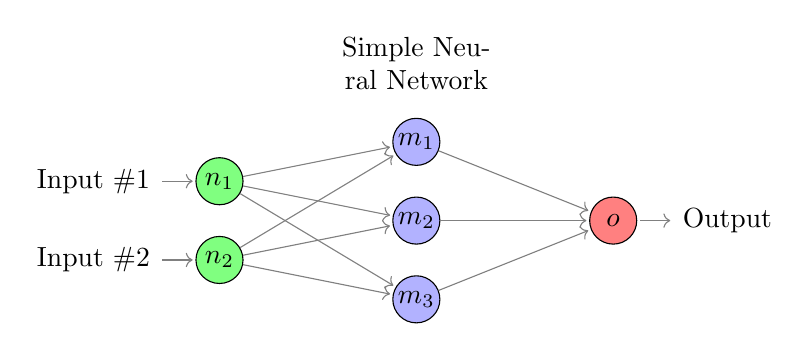
\begin{tikzpicture}[shorten >=1pt,->,draw=black!50, node distance=\layersep]
%https://tex.stackexchange.com/questions/96846/how-to-place-label-in-middle-of-line-above-and-below-with-tikz
    \tikzstyle{every pin edge}=[<-,shorten <=1pt]
    \tikzstyle{neuron}=[circle,fill=black!25,minimum size=17pt,inner sep=0pt, draw=black]
    \tikzstyle{input neuron}=[neuron, fill=green!50];
    \tikzstyle{output neuron}=[neuron, fill=red!50];
    \tikzstyle{hidden neuron}=[neuron, fill=blue!30];
    \tikzstyle{annot} = [text width=10em, text centered]

    % Draw the input layer nodes
    \foreach \name / \y in {1,...,2}
    % This is the same as writing \foreach \name / \y in {1/1,2/2,3/3,4/4}
        \node[input neuron, pin=left:Input \#\y] (I-\name) at (0,-\y) {$n_\y$};

    % Draw the hidden layer nodes
    \foreach \name / \y in {1,...,3}
        \path[yshift=0.5cm]
            node[hidden neuron] (H-\name) at (\layersep,-\y cm) {$m_\y$};

    % Draw the output layer node
    \node[output neuron,pin={[pin edge={->}]right:Output}, right of=H-2] (O) {$o$};

    % Connect every node in the input layer with every node in the
    % hidden layer.
%    \foreach \source in {1,...,4}
%        \foreach \dest in {1,...,5}
%            \draw (I-\source) -- node[below] {$w_ij$} ++ (H-\dest);


    \foreach \source in {1,...,2}
        \foreach \dest in {1,...,3}
		  \draw (I-\source) -- (H-\dest);
%            \draw (I-2) -- node[above, pos=0.8] {$w_{2\dest}$} ++ (H-\dest);

    % Connect every node in the hidden layer with the output layer
    \foreach \source in {1,...,3}
        \path (H-\source) edge (O);
    \node[annot,above of=H-1, node distance=1cm] (hl) {Simple Neural Network};
\end{tikzpicture}
  \end{minipage}
  \vfill
\begin{minipage}[t][0.5\textheight][t]{\textwidth}
In 1949, psychologist Donald Hebb pointed out the neural pathways are strengthened each time they were used, a concept which gave a potential mechanism to human learning. Practically, this means that each of the edges connecting the nodes can carry a multiplicitive weight which appropriately scales the input. 
\end{minipage}
\end{frame}




\begin{frame}[fragile]{Towards Modern Neurons}
  \begin{minipage}[t][0.5\textheight][t]{\textwidth}
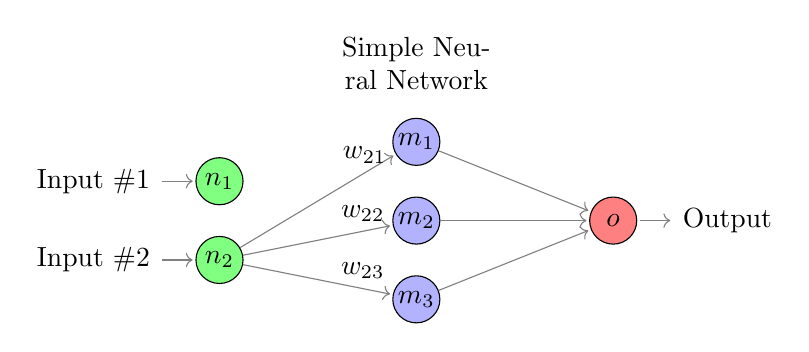
\begin{tikzpicture}[shorten >=1pt,->,draw=black!50, node distance=\layersep]
%https://tex.stackexchange.com/questions/96846/how-to-place-label-in-middle-of-line-above-and-below-with-tikz
    \tikzstyle{every pin edge}=[<-,shorten <=1pt]
    \tikzstyle{neuron}=[circle,fill=black!25,minimum size=17pt,inner sep=0pt, draw=black]
    \tikzstyle{input neuron}=[neuron, fill=green!50];
    \tikzstyle{output neuron}=[neuron, fill=red!50];
    \tikzstyle{hidden neuron}=[neuron, fill=blue!30];
    \tikzstyle{annot} = [text width=10em, text centered]

    % Draw the input layer nodes
    \foreach \name / \y in {1,...,2}
    % This is the same as writing \foreach \name / \y in {1/1,2/2,3/3,4/4}
        \node[input neuron, pin=left:Input \#\y] (I-\name) at (0,-\y) {$n_\y$};

    % Draw the hidden layer nodes
    \foreach \name / \y in {1,...,3}
        \path[yshift=0.5cm]
            node[hidden neuron] (H-\name) at (\layersep,-\y cm) {$m_\y$};

    % Draw the output layer node
    \node[output neuron,pin={[pin edge={->}]right:Output}, right of=H-2] (O) {$o$};

    % Connect every node in the input layer with every node in the
    % hidden layer.
%    \foreach \source in {1,...,4}
%        \foreach \dest in {1,...,5}
%            \draw (I-\source) -- node[below] {$w_ij$} ++ (H-\dest);


%    \foreach \source in {1,...,2}
        \foreach \dest in {1,...,3}
%		  \draw (I-\source) -- (H-\dest);
            \draw (I-2) -- node[above, pos=0.8] {$w_{2\dest}$} ++ (H-\dest);

    % Connect every node in the hidden layer with the output layer
    \foreach \source in {1,...,3}
        \path (H-\source) edge (O);
    \node[annot,above of=H-1, node distance=1cm] (hl) {Simple Neural Network};
\end{tikzpicture}
  \end{minipage}
  \vfill
\begin{minipage}[t][0.5\textheight][t]{\textwidth}
While the output was still binary, the weights allowed the connections to be evaluated non-symmetrically. \pause In addition to the weights, these early neural networks incorporated a \textbf{Bayesian} firing mechanisms. \pause Both the weights and the firing probability were increased each time the pair of nodes successfully fired. 
\end{minipage}
\end{frame}




\begin{frame}[fragile]{Towards Modern Neurons}
  \begin{minipage}[t][0.5\textheight][t]{\textwidth}
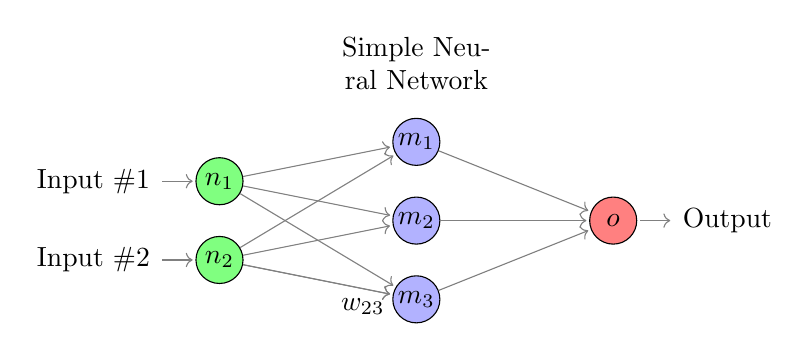
\begin{tikzpicture}[shorten >=1pt,->,draw=black!50, node distance=\layersep]
%https://tex.stackexchange.com/questions/96846/how-to-place-label-in-middle-of-line-above-and-below-with-tikz
    \tikzstyle{every pin edge}=[<-,shorten <=1pt]
    \tikzstyle{neuron}=[circle,fill=black!25,minimum size=17pt,inner sep=0pt, draw=black]
    \tikzstyle{input neuron}=[neuron, fill=green!50];
    \tikzstyle{output neuron}=[neuron, fill=red!50];
    \tikzstyle{hidden neuron}=[neuron, fill=blue!30];
    \tikzstyle{annot} = [text width=10em, text centered]

    % Draw the input layer nodes
    \foreach \name / \y in {1,...,2}
    % This is the same as writing \foreach \name / \y in {1/1,2/2,3/3,4/4}
        \node[input neuron, pin=left:Input \#\y] (I-\name) at (0,-\y) {$n_\y$};

    % Draw the hidden layer nodes
    \foreach \name / \y in {1,...,3}
        \path[yshift=0.5cm]
            node[hidden neuron] (H-\name) at (\layersep,-\y cm) {$m_\y$};

    % Draw the output layer node
    \node[output neuron,pin={[pin edge={->}]right:Output}, right of=H-2] (O) {$o$};

    % Connect every node in the input layer with every node in the
    % hidden layer.
%    \foreach \source in {1,...,4}
%        \foreach \dest in {1,...,5}
%            \draw (I-\source) -- node[below] {$w_ij$} ++ (H-\dest);


    \foreach \source in {1,...,2}
        \foreach \dest in {1,...,3}
		  \draw (I-\source) -- (H-\dest);
%            \draw (I-2) -- node[above, pos=0.8] {$w_{2\dest}$} ++ (H-\dest);

	\draw (I-2) -- node[below, pos=0.8] {$w_{23}$} ++ (H-3);

    % Connect every node in the hidden layer with the output layer
    \foreach \source in {1,...,3}
        \path (H-\source) edge (O);
    \node[annot,above of=H-1, node distance=1cm] (hl) {Simple Neural Network};
\end{tikzpicture}
  \end{minipage}
  \vfill
\begin{minipage}[t][0.5\textheight][t]{\textwidth}
While the output was still binary, the weights allowed the connections to be evaluated non-symmetrically.  In addition to the weights, these early neural networks incorporated a \textbf{Bayesian} firing mechanisms. Both the weights and the firing probability were increased each time the pair of nodes successfully fired. 
\end{minipage}
\end{frame}




\begin{frame}[fragile]{Towards Modern Neurons}
  \begin{minipage}[t][0.5\textheight][t]{\textwidth}
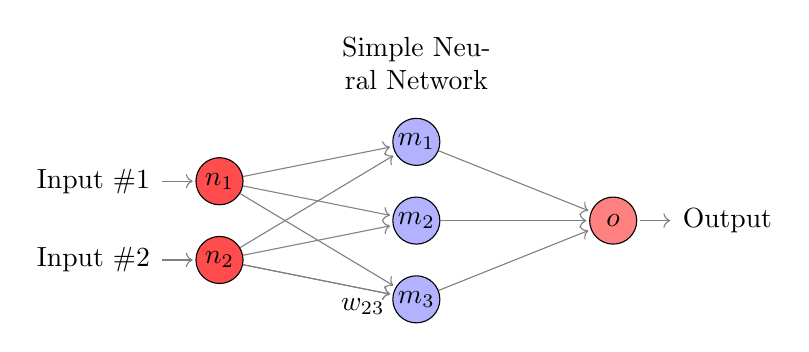
\begin{tikzpicture}[shorten >=1pt,->,draw=black!50, node distance=\layersep]
%https://tex.stackexchange.com/questions/96846/how-to-place-label-in-middle-of-line-above-and-below-with-tikz
    \tikzstyle{every pin edge}=[<-,shorten <=1pt]
    \tikzstyle{neuron}=[circle,fill=black!25,minimum size=17pt,inner sep=0pt, draw=black]
    \tikzstyle{input neuron}=[neuron, fill=red!70];
    \tikzstyle{output neuron}=[neuron, fill=red!50];
    \tikzstyle{hidden neuron}=[neuron, fill=blue!30];
    \tikzstyle{annot} = [text width=10em, text centered]

    % Draw the input layer nodes
    \foreach \name / \y in {1,...,2}
    % This is the same as writing \foreach \name / \y in {1/1,2/2,3/3,4/4}
        \node[input neuron, pin=left:Input \#\y] (I-\name) at (0,-\y) {$n_\y$};

    % Draw the hidden layer nodes
    \foreach \name / \y in {1,...,3}
        \path[yshift=0.5cm]
            node[hidden neuron] (H-\name) at (\layersep,-\y cm) {$m_\y$};

    % Draw the output layer node
    \node[output neuron,pin={[pin edge={->}]right:Output}, right of=H-2] (O) {$o$};

    % Connect every node in the input layer with every node in the
    % hidden layer.
%    \foreach \source in {1,...,4}
%        \foreach \dest in {1,...,5}
%            \draw (I-\source) -- node[below] {$w_ij$} ++ (H-\dest);


    \foreach \source in {1,...,2}
        \foreach \dest in {1,...,3}
		  \draw (I-\source) -- (H-\dest);
%            \draw (I-2) -- node[above, pos=0.8] {$w_{2\dest}$} ++ (H-\dest);

	\draw (I-2) -- node[below, pos=0.8] {$w_{23}$} ++ (H-3);

    % Connect every node in the hidden layer with the output layer
    \foreach \source in {1,...,3}
        \path (H-\source) edge (O);
    \node[annot,above of=H-1, node distance=1cm] (hl) {Simple Neural Network};
\end{tikzpicture}
  \end{minipage}
  \vfill
\begin{minipage}[t][0.5\textheight][t]{\textwidth}
While the output was still binary, the weights allowed the connections to be evaluated non-symmetrically.  In addition to the weights, these early neural networks incorporated a \textbf{Bayesian} firing mechanisms. Both the weights and the firing probability were increased each time the pair of nodes successfully fired. 
\end{minipage}
\end{frame}




\begin{frame}[fragile]{Towards Modern Neurons}
  \begin{minipage}[t][0.5\textheight][t]{\textwidth}
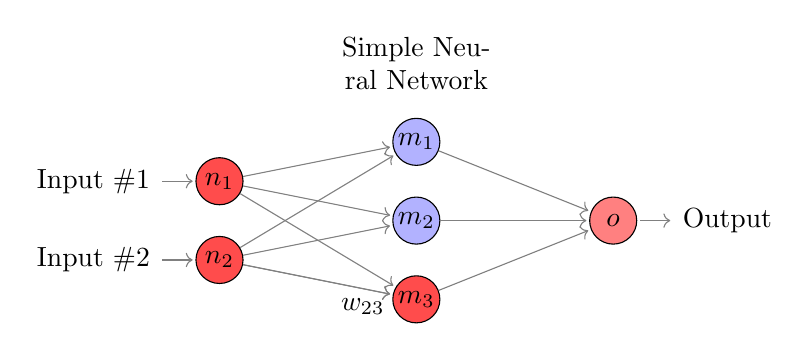
\begin{tikzpicture}[shorten >=1pt,->,draw=black!50, node distance=\layersep]
%https://tex.stackexchange.com/questions/96846/how-to-place-label-in-middle-of-line-above-and-below-with-tikz
    \tikzstyle{every pin edge}=[<-,shorten <=1pt]
    \tikzstyle{neuron}=[circle,fill=black!25,minimum size=17pt,inner sep=0pt, draw=black]
    \tikzstyle{input neuron}=[neuron, fill=red!70];
    \tikzstyle{output neuron}=[neuron, fill=red!50];
    \tikzstyle{hidden neuron}=[neuron, fill=blue!30];
    \tikzstyle{annot} = [text width=10em, text centered]

    % Draw the input layer nodes
    \foreach \name / \y in {1,...,2}
    % This is the same as writing \foreach \name / \y in {1/1,2/2,3/3,4/4}
        \node[input neuron, pin=left:Input \#\y] (I-\name) at (0,-\y) {$n_\y$};

    % Draw the hidden layer nodes
    \foreach \name / \y in {1,...,2}
        \path[yshift=0.5cm]
            node[hidden neuron] (H-\name) at (\layersep,-\y cm) {$m_\y$};

    \node[hidden neuron, fill=red!70] (H-3) at (\layersep,-2.5 cm) {$m_3$};

    % Draw the output layer node
    \node[output neuron,pin={[pin edge={->}]right:Output}, right of=H-2] (O) {$o$};

    % Connect every node in the input layer with every node in the
    % hidden layer.
%    \foreach \source in {1,...,4}
%        \foreach \dest in {1,...,5}
%            \draw (I-\source) -- node[below] {$w_ij$} ++ (H-\dest);


    \foreach \source in {1,...,2}
        \foreach \dest in {1,...,3}
		  \draw (I-\source) -- (H-\dest);
%            \draw (I-2) -- node[above, pos=0.8] {$w_{2\dest}$} ++ (H-\dest);

	\draw (I-2) -- node[below, pos=0.8] {$w_{23}$} ++ (H-3);

    % Connect every node in the hidden layer with the output layer
    \foreach \source in {1,...,3}
        \path (H-\source) edge (O);
    \node[annot,above of=H-1, node distance=1cm] (hl) {Simple Neural Network};
\end{tikzpicture}
  \end{minipage}
  \vfill
\begin{minipage}[t][0.5\textheight][t]{\textwidth}
While the output was still binary, the weights allowed the connections to be evaluated non-symmetrically.  In addition to the weights, these early neural networks incorporated a \textbf{Bayesian} firing mechanisms. Both the weights and the firing probability were increased each time the pair of nodes successfully fired. 
\end{minipage}
\end{frame}




\begin{frame}[fragile]{Towards Modern Neurons}
  \begin{minipage}[t][0.5\textheight][t]{\textwidth}
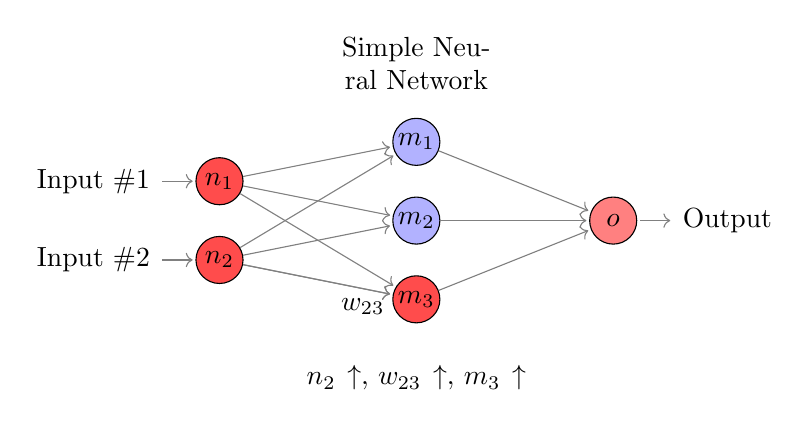
\begin{tikzpicture}[shorten >=1pt,->,draw=black!50, node distance=\layersep]
%https://tex.stackexchange.com/questions/96846/how-to-place-label-in-middle-of-line-above-and-below-with-tikz
    \tikzstyle{every pin edge}=[<-,shorten <=1pt]
    \tikzstyle{neuron}=[circle,fill=black!25,minimum size=17pt,inner sep=0pt, draw=black]
    \tikzstyle{input neuron}=[neuron, fill=red!70];
    \tikzstyle{output neuron}=[neuron, fill=red!50];
    \tikzstyle{hidden neuron}=[neuron, fill=blue!30];
    \tikzstyle{annot} = [text width=10em, text centered]

    % Draw the input layer nodes
    \foreach \name / \y in {1,...,2}
    % This is the same as writing \foreach \name / \y in {1/1,2/2,3/3,4/4}
        \node[input neuron, pin=left:Input \#\y] (I-\name) at (0,-\y) {$n_\y$};

    % Draw the hidden layer nodes
    \foreach \name / \y in {1,...,2}
        \path[yshift=0.5cm]
            node[hidden neuron] (H-\name) at (\layersep,-\y cm) {$m_\y$};

    \node[hidden neuron, fill=red!70] (H-3) at (\layersep,-2.5 cm) {$m_3$};

    % Draw the output layer node
    \node[output neuron,pin={[pin edge={->}]right:Output}, right of=H-2] (O) {$o$};

    % Connect every node in the input layer with every node in the
    % hidden layer.
%    \foreach \source in {1,...,4}
%        \foreach \dest in {1,...,5}
%            \draw (I-\source) -- node[below] {$w_ij$} ++ (H-\dest);


    \foreach \source in {1,...,2}
        \foreach \dest in {1,...,3}
		  \draw (I-\source) -- (H-\dest);
%            \draw (I-2) -- node[above, pos=0.8] {$w_{2\dest}$} ++ (H-\dest);

	\draw (I-2) -- node[below, pos=0.8] {$w_{23}$} ++ (H-3);

    \node[annot,below of=H-3, node distance=1cm] (hl) {$n_2\uparrow, \, w_{23}\uparrow,\, m_3\uparrow$};

    % Connect every node in the hidden layer with the output layer
    \foreach \source in {1,...,3}
        \path (H-\source) edge (O);
    \node[annot,above of=H-1, node distance=1cm] (hl) {Simple Neural Network};
\end{tikzpicture}
  \end{minipage}
  \vfill
\begin{minipage}[t][0.5\textheight][t]{\textwidth}
Here, $n_i$ and $m_j$ represent the firing probabilities. In addition, $n_1$ and $w_{13}$ would increase in this model. 
\end{minipage}
\end{frame}





\section{Linear Classifier, Neural Networks and the Perceptron}






\begin{frame}[fragile]{Towards Modern Neurons}
  \begin{minipage}[t][0.5\textheight][t]{\textwidth}
  \centering \includegraphics[height=0.5\textheight]{L11PerceptronMachine.png} 
  \end{minipage}
  \vfill
\begin{minipage}[t][0.5\textheight][t]{\textwidth}
In 1957 Frank Rosenblatt introduced a linear algorithm into the ANN literature called the Perceptron.  The perceptron actually entered the world as a hardware device, not as a software algorithms.\newline \pause

In 1957 Frank Rosenblatt introduced a linear algorithm into the ANN literature called the Perceptron.  The perceptron is based around a \textbf{linear threshold unit} (\textbf{LTU}).
\end{minipage}
\end{frame}








\begin{frame}[fragile]{Perceptron}
  \begin{minipage}[t][0.5\textheight][t]{\textwidth}
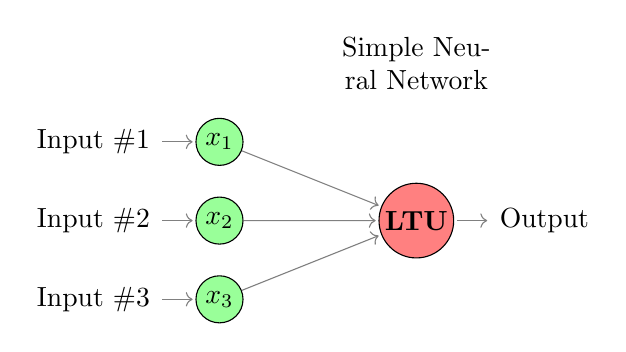
\begin{tikzpicture}[shorten >=1pt,->,draw=black!50, node distance=\layersep]
%https://tex.stackexchange.com/questions/96846/how-to-place-label-in-middle-of-line-above-and-below-with-tikz
    \tikzstyle{every pin edge}=[<-,shorten <=1pt]
    \tikzstyle{neuron}=[circle,fill=black!25,minimum size=17pt,inner sep=0pt, draw=black]
    \tikzstyle{input neuron}=[neuron, fill=green!40];
    \tikzstyle{output neuron}=[neuron, fill=red!50];
    \tikzstyle{hidden neuron}=[neuron, fill=blue!30];
    \tikzstyle{annot} = [text width=10em, text centered]

    % Draw the input layer nodes
    \foreach \name / \y in {1,...,3}
    % This is the same as writing \foreach \name / \y in {1/1,2/2,3/3,4/4}
        \node[input neuron, pin=left:Input \#\y] (I-\name) at (0,-\y) {$x_\y$};

    % Draw the hidden layer nodes
        \node[output neuron, pin={[pin edge={->}]right:Output}] (H-1) at (\layersep,- 2cm) {$\,\textbf{LTU}\,$};

    \foreach \source in {1,...,3}
        \foreach \dest in {1,...,1}
		  \draw (I-\source) -- (H-\dest);


    \node[annot,above of=H-1, node distance=2cm] (hl) {Simple Neural Network};
\end{tikzpicture}
  \end{minipage}
  \vfill
\begin{minipage}[t][0.5\textheight][t]{\textwidth}
The LTU sums the inputs and then applies a step function:
$$
\textbf{LTU}: y = \text{step}(w_1x_1+ w_2x_2+\ldots +w_px_p)\,,
$$\pause
where $\text{step}(x)$ is the Heaviside step function. 
$$
\text{step}(x) = \begin{cases}
0&\text{if } x < 0\,,
\\
1&\text{if } x\geq 0\,.
\end{cases}
$$\,.

\end{minipage}
\end{frame}




\begin{frame}[fragile]{Perceptron}
  \begin{minipage}[t][0.5\textheight][t]{\textwidth}
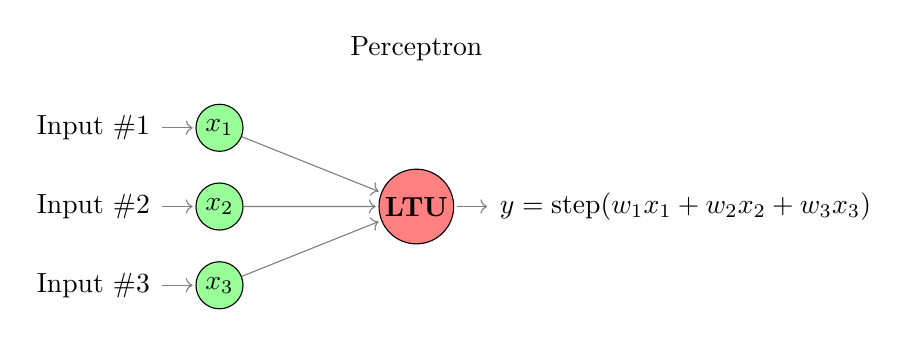
\begin{tikzpicture}[shorten >=1pt,->,draw=black!50, node distance=\layersep]
%https://tex.stackexchange.com/questions/96846/how-to-place-label-in-middle-of-line-above-and-below-with-tikz
    \tikzstyle{every pin edge}=[<-,shorten <=1pt]
    \tikzstyle{neuron}=[circle,fill=black!25,minimum size=17pt,inner sep=0pt, draw=black]
    \tikzstyle{input neuron}=[neuron, fill=green!40];
    \tikzstyle{output neuron}=[neuron, fill=red!50];
    \tikzstyle{hidden neuron}=[neuron, fill=blue!30];
    \tikzstyle{annot} = [text width=10em, text centered]

    % Draw the input layer nodes
    \foreach \name / \y in {1,...,3}
    % This is the same as writing \foreach \name / \y in {1/1,2/2,3/3,4/4}
        \node[input neuron, pin=left:Input \#\y] (I-\name) at (0,-\y) {$x_\y$};
        

    % Draw the hidden layer nodes
        \node[output neuron, pin={[pin edge={->}]right: $y=\text{step}(w_1x_1+w_2x_2+ w_3x_3)$ }] (H-1) at (\layersep,- 2cm) {$\,\textbf{LTU}\,$};

    \foreach \source in {1,...,3}
        \foreach \dest in {1,...,1}
		  \draw (I-\source) -- (H-\dest);


    \node[annot,above of=H-1, node distance=2cm] (hl) {Perceptron};
\end{tikzpicture}
  \end{minipage}
  \vfill
\begin{minipage}[t][0.5\textheight][t]{\textwidth}
A single LTU gives a binary classifier using the sum of linear functions. Notice that functionally this give the same hypothesis class as (non-affine) linear regression
$$
y =  \text{step}(x_{1}\beta_1 + \ldots +  x_{p}\beta_p)
$$
\end{minipage}
\end{frame}







\begin{frame}[fragile]{Perceptron}
  \begin{minipage}[t][0.5\textheight][t]{\textwidth}
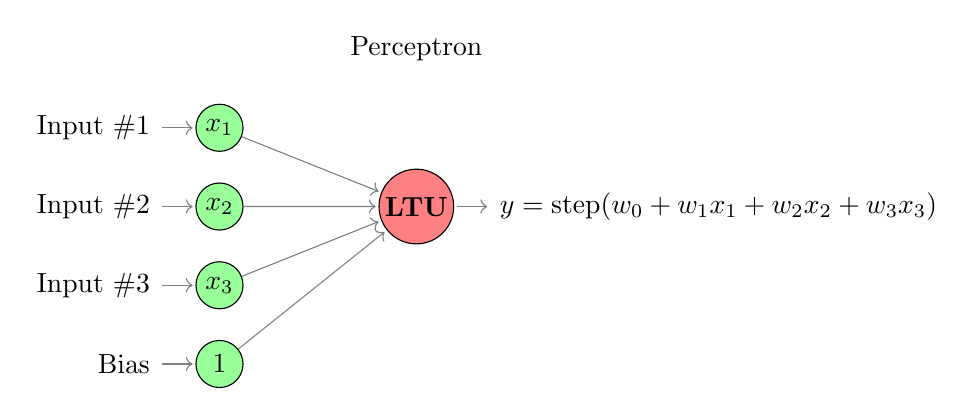
\begin{tikzpicture}[shorten >=1pt,->,draw=black!50, node distance=\layersep]
%https://tex.stackexchange.com/questions/96846/how-to-place-label-in-middle-of-line-above-and-below-with-tikz
    \tikzstyle{every pin edge}=[<-,shorten <=1pt]
    \tikzstyle{neuron}=[circle,fill=black!25,minimum size=17pt,inner sep=0pt, draw=black]
    \tikzstyle{input neuron}=[neuron, fill=green!40];
    \tikzstyle{output neuron}=[neuron, fill=red!50];
    \tikzstyle{hidden neuron}=[neuron, fill=blue!30];
    \tikzstyle{annot} = [text width=10em, text centered]

    % Draw the input layer nodes
    \foreach \name / \y in {1,...,3}
    % This is the same as writing \foreach \name / \y in {1/1,2/2,3/3,4/4}
        \node[input neuron, pin=left:Input \#\y] (I-\name) at (0,-\y) {$x_\y$};
        
    \foreach \name / \y in {4}
    % This is the same as writing \foreach \name / \y in {1/1,2/2,3/3,4/4}
        \node[input neuron, pin=left:Bias] (I-\name) at (0,-\y) {$1$};

    % Draw the hidden layer nodes
        \node[output neuron, pin={[pin edge={->}]right: $y=\text{step}(w_0+w_1x_1+w_2x_2+ w_3x_3)$ }] (H-1) at (\layersep,- 2cm) {$\,\textbf{LTU}\,$};
        
        

    \foreach \source in {1,...,4}
        \foreach \dest in {1,...,1}
		  \draw (I-\source) -- (H-\dest);


    \node[annot,above of=H-1, node distance=2cm] (hl) {Perceptron};
\end{tikzpicture}
  \end{minipage}
  \vfill
\begin{minipage}[t][0.5\textheight][t]{\textwidth}
Finally, we can add a constant bias neuron to produce the affine terms $w_{0}$. We see that our perceptron can be used to perform categorical linear regression for binary classification.
$$
y =  \text{step}(\beta_0 + x_{1}\beta_1 + \ldots +  x_{p}\beta_p)\,.
$$

\end{minipage}
\end{frame}





\begin{frame}[fragile]{Perceptron}
  \begin{minipage}[t][0.5\textheight][t]{\textwidth}
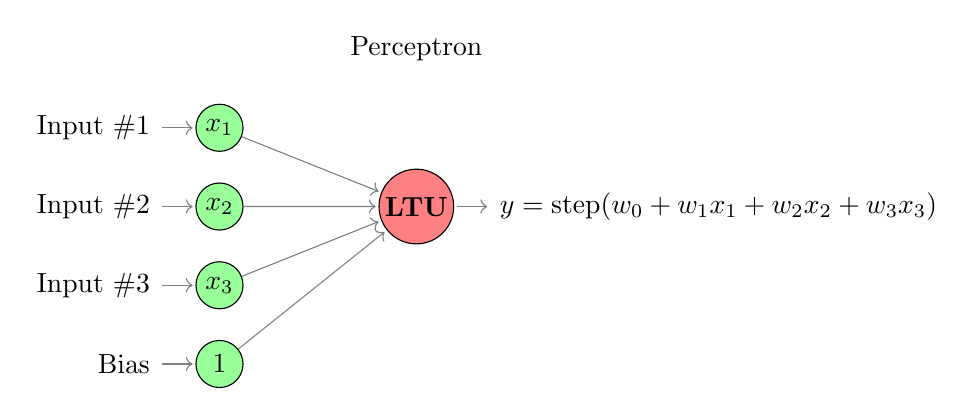
\begin{tikzpicture}[shorten >=1pt,->,draw=black!50, node distance=\layersep]
%https://tex.stackexchange.com/questions/96846/how-to-place-label-in-middle-of-line-above-and-below-with-tikz
    \tikzstyle{every pin edge}=[<-,shorten <=1pt]
    \tikzstyle{neuron}=[circle,fill=black!25,minimum size=17pt,inner sep=0pt, draw=black]
    \tikzstyle{input neuron}=[neuron, fill=green!40];
    \tikzstyle{output neuron}=[neuron, fill=red!50];
    \tikzstyle{hidden neuron}=[neuron, fill=blue!30];
    \tikzstyle{annot} = [text width=10em, text centered]

    % Draw the input layer nodes
    \foreach \name / \y in {1,...,3}
    % This is the same as writing \foreach \name / \y in {1/1,2/2,3/3,4/4}
        \node[input neuron, pin=left:Input \#\y] (I-\name) at (0,-\y) {$x_\y$};
        
    \foreach \name / \y in {4}
    % This is the same as writing \foreach \name / \y in {1/1,2/2,3/3,4/4}
        \node[input neuron, pin=left:Bias] (I-\name) at (0,-\y) {$1$};

    % Draw the hidden layer nodes
        \node[output neuron, pin={[pin edge={->}]right: $y=\text{step}(w_0+w_1x_1+w_2x_2+ w_3x_3)$ }] (H-1) at (\layersep,- 2cm) {$\,\textbf{LTU}\,$};
        
        

    \foreach \source in {1,...,4}
        \foreach \dest in {1,...,1}
		  \draw (I-\source) -- (H-\dest);


    \node[annot,above of=H-1, node distance=2cm] (hl) {Perceptron};
\end{tikzpicture}
  \end{minipage}
  \vfill
\begin{minipage}[t][0.5\textheight][t]{\textwidth}
In a modern neural network, we follow the following terminology:
\begin{itemize}
\item \textbf{Nodes}: Data holding variables. 
\item \textbf{Input Nodes}: A set of $p$ nodes in which we feed the $x_i$, either for training or prediction. Here, $p$ is the number of features for each input vector. 
\item \textbf{Bias Node}: A constant node. 
\end{itemize}
\end{minipage}
\end{frame}

\begin{frame}[fragile]{Perceptron}
  \begin{minipage}[t][0.5\textheight][t]{\textwidth}
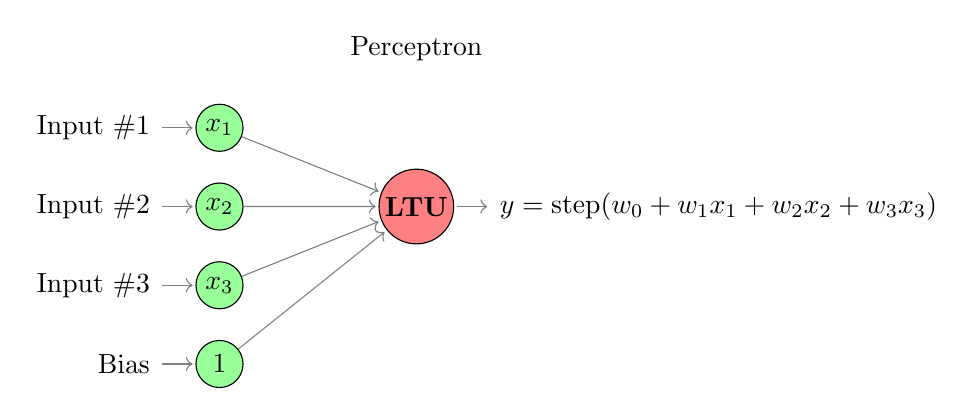
\begin{tikzpicture}[shorten >=1pt,->,draw=black!50, node distance=\layersep]
%https://tex.stackexchange.com/questions/96846/how-to-place-label-in-middle-of-line-above-and-below-with-tikz
    \tikzstyle{every pin edge}=[<-,shorten <=1pt]
    \tikzstyle{neuron}=[circle,fill=black!25,minimum size=17pt,inner sep=0pt, draw=black]
    \tikzstyle{input neuron}=[neuron, fill=green!40];
    \tikzstyle{output neuron}=[neuron, fill=red!50];
    \tikzstyle{hidden neuron}=[neuron, fill=blue!30];
    \tikzstyle{annot} = [text width=10em, text centered]

    % Draw the input layer nodes
    \foreach \name / \y in {1,...,3}
    % This is the same as writing \foreach \name / \y in {1/1,2/2,3/3,4/4}
        \node[input neuron, pin=left:Input \#\y] (I-\name) at (0,-\y) {$x_\y$};
        
    \foreach \name / \y in {4}
    % This is the same as writing \foreach \name / \y in {1/1,2/2,3/3,4/4}
        \node[input neuron, pin=left:Bias] (I-\name) at (0,-\y) {$1$};

    % Draw the hidden layer nodes
        \node[output neuron, pin={[pin edge={->}]right: $y=\text{step}(w_0+w_1x_1+w_2x_2+ w_3x_3)$ }] (H-1) at (\layersep,- 2cm) {$\,\textbf{LTU}\,$};
        
        

    \foreach \source in {1,...,4}
        \foreach \dest in {1,...,1}
		  \draw (I-\source) -- (H-\dest);


    \node[annot,above of=H-1, node distance=2cm] (hl) {Perceptron};
\end{tikzpicture}
  \end{minipage}
  \vfill
\begin{minipage}[t][0.5\textheight][t]{\textwidth}
In a modern neural network, we follow the following terminology:
\begin{itemize}
\item \textbf{Edges}: Each edge connects two nodes and carries a \textbf{weight} $w$. A weight is a trainable constant parameter of the network. 
\item \textbf{Output Node}: Output nodes each hold a single dimension of a $K$ dimensional output $Y$.
\end{itemize}
\end{minipage}
\end{frame}





\begin{frame}[fragile]{Perceptron}
  \begin{minipage}[t][0.5\textheight][t]{\textwidth}
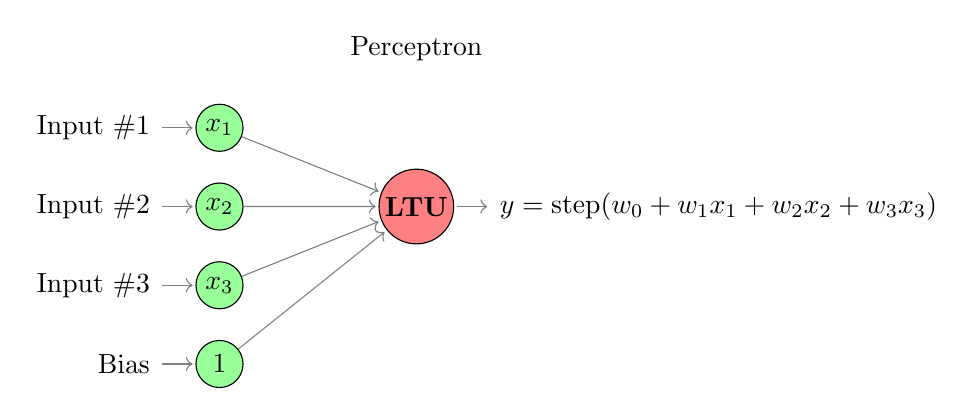
\begin{tikzpicture}[shorten >=1pt,->,draw=black!50, node distance=\layersep]
%https://tex.stackexchange.com/questions/96846/how-to-place-label-in-middle-of-line-above-and-below-with-tikz
    \tikzstyle{every pin edge}=[<-,shorten <=1pt]
    \tikzstyle{neuron}=[circle,fill=black!25,minimum size=17pt,inner sep=0pt, draw=black]
    \tikzstyle{input neuron}=[neuron, fill=green!40];
    \tikzstyle{output neuron}=[neuron, fill=red!50];
    \tikzstyle{hidden neuron}=[neuron, fill=blue!30];
    \tikzstyle{annot} = [text width=10em, text centered]

    % Draw the input layer nodes
    \foreach \name / \y in {1,...,3}
    % This is the same as writing \foreach \name / \y in {1/1,2/2,3/3,4/4}
        \node[input neuron, pin=left:Input \#\y] (I-\name) at (0,-\y) {$x_\y$};
        
    \foreach \name / \y in {4}
    % This is the same as writing \foreach \name / \y in {1/1,2/2,3/3,4/4}
        \node[input neuron, pin=left:Bias] (I-\name) at (0,-\y) {$1$};

    % Draw the hidden layer nodes
        \node[output neuron, pin={[pin edge={->}]right: $y=\text{step}(w_0+w_1x_1+w_2x_2+ w_3x_3)$ }] (H-1) at (\layersep,- 2cm) {$\,\textbf{LTU}\,$};
        
        

    \foreach \source in {1,...,4}
        \foreach \dest in {1,...,1}
		  \draw (I-\source) -- (H-\dest);


    \node[annot,above of=H-1, node distance=2cm] (hl) {Perceptron};
\end{tikzpicture}
  \end{minipage}
  \vfill
\begin{minipage}[t][0.5\textheight][t]{\textwidth}
In a modern neural network, we follow the following terminology:
\begin{itemize}
\item \textbf{LTU:} An LTU node takes and holds the sum over all inputing nodes, weighted by the edge weighting. It then compose that linear combination with an \textbf{activation function} to restrict the value range. For the perceptron, the activation function is $\textbf{step}$.
\end{itemize}
\end{minipage}
\end{frame}





\begin{frame}[fragile]{Perception}
\textbf{Training the Perceptron}: Write the perceptron function as

$$
w_0+w_1X_1+\ldots+ w_pX_p = w^TX= \langle w, X\rangle\,.
$$

Initially, set all $w^{(0)}=0$. At each step the, perception randomly samples a point $x_i$ and predicts a label $\hat{y}_i$ based on $w^{(j)}$. \pause We then update to $w^{(j+1)}$ by computing
$$
w^{(j+1)} = w^{(j)} + (y_i - \hat{y}_i)x_i\,.
$$ \pause
If $\hat{y}_i = y_i$, the point is correctly classified and we move on. But if $y_i \neq \hat{y}_i$, then 
$$
(y_i - \hat{y}_i) = \begin{cases}
1 &\text{if } \hat{y}_i=0\,,
\\
-1 &\text{if } \hat{y}_i=1\,.
\end{cases}
$$ 

\end{frame}





\begin{frame}[fragile]{Perception}
We want to see that the new weights 
$$
w^{(j+1)} = w^{(j)} + (y_i - \hat{y}_i)x_i\,.
$$
classify $y_i$ better than the old weights. Notice that 
$$
\hat{y} = \begin{cases}
0 &\text{if } \langle w, x_i\rangle<0\,,
\\
1 &\text{if } \langle w, x_i\rangle>0\,.
\end{cases}
$$
So this means that if $y_i \neq \hat{y}_i$ then 
$$
(y-\hat{y})\langle w^{(j)}, x_i\rangle<0\,.
$$
So improving our guess for $y_i$ means increasing $\langle w, x_i\rangle$ if $y_i=1$, or decreasing it if $y_i=0$. Either way, we will have been successful if 
$$
(y_i-\hat{y}_i)\langle w^{(j+1)}, x_i\rangle > (y_i-\hat{y}_i)\langle w^{(j)}, x_i\rangle 
$$

\end{frame}


\begin{frame}[fragile]{Perception}
It not too hard to see that this will be the case:
\begin{align*}
(y_i-\hat{y}_i)\langle w^{(j+1)}, x_i\rangle &= (y-\hat{y})\langle w^{(j)} + (y_i - \hat{y}_i)x_i , x_i\rangle 
\\
&=
(y-\hat{y}) w^{(j)} + ||x_i||^2
\\
&>(y-\hat{y}) w^{(j)}\,.
\end{align*}
The new halfplane "more correctly" classifies $x_i$. The algorithm stops when all points are classified. 
\url{https://www.youtube.com/watch?v=xpJHhHwR4DQ}
\end{frame}





\begin{frame}[fragile]{Perception}
\textbf{Theorem:} Assume that $(x_i,y_i)$ are separable. Let $R = \text{max}_i||x_i||$ be roughly the data size and
$$
B = \min\{||\beta||\,:\,y_i\langle  x_i,\beta\rangle\geq 1\,\forall i\}
$$
be roughly the gap distance. Then the perceptron algorithm stops after at most $(RB)^2$ iterations. \pause

A couple of points about the perceptron:
\begin{itemize}
\item[] When the data is separable, there are many solutions and which one is found depends on the starting value. \pause
\item[] The finite number of steps can be large, practically, if the gap is small the time to find it is large. \pause
\item[] When the data are not seperable, the algorithm does not converge, and instead falls into a cycle. 
\end{itemize}
\end{frame}




\begin{frame}[fragile]{Perception}
The perceptron is a form of stochastic gradient decent on the loss function
$$
\ell(w) = -\sum_{i=1}^N (y_i-\hat{y}_i)(x_i^Tw)\,.
$$
Notice that this loss is non-negative, and only 0 when all labels $\hat{y}$ are correctly fitted.\pause The gradient is
$$
\frac{\partial\ell}{\partial w} = -\sum_{i=1}^N (y_i-\hat{y}_i) x_i\,.
$$\pause
In gradient decent, we would update $w$ and using the full gradient,
$$
w = w + \eta \sum_{i=1}^N (y_i-\hat{y}_i) x_i\,,
$$
but here we are making the SGD update on the single datapoint $(x_i, y_i)$:
$$
w = w +  (y_i-\hat{y}_i) x_i\,.
$$
\end{frame}



\begin{frame}[fragile]{Perception}
  \begin{minipage}[t][0.5\textheight][t]{\textwidth}
	\centering \includegraphics[height=0.5\textheight]{L9StocGradDecent.png} 
  \end{minipage}
  \vfill
\begin{minipage}[t][0.5\textheight][t]{\textwidth}
Completing the conversion to Stochasitic gradient decent, we add in a learning parameter $\eta$:
$$
w = w +  (y_i-\hat{y}_i) x_i\,.
$$
\end{minipage}
\end{frame}






\section{Multilabel Perceptrons}



\begin{frame}[fragile]{Perceptron}
  \begin{minipage}[t][0.5\textheight][t]{\textwidth}
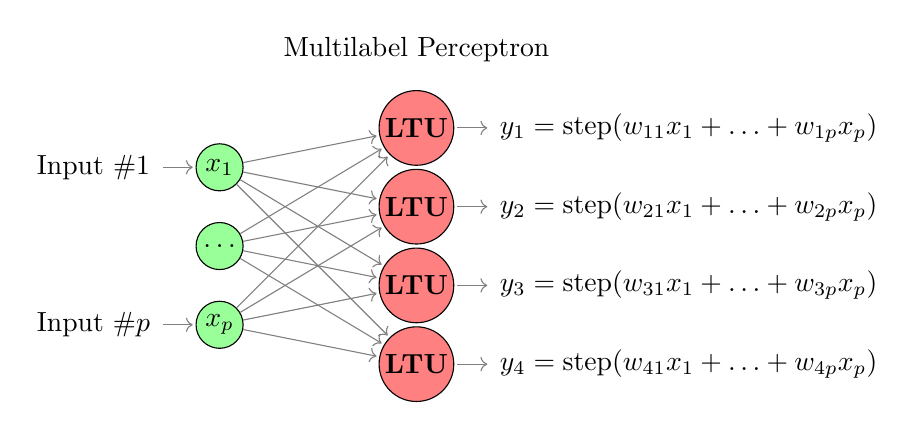
\begin{tikzpicture}[shorten >=1pt,->,draw=black!50, node distance=\layersep]
%https://tex.stackexchange.com/questions/96846/how-to-place-label-in-middle-of-line-above-and-below-with-tikz
    \tikzstyle{every pin edge}=[<-,shorten <=1pt]
    \tikzstyle{neuron}=[circle,fill=black!25,minimum size=17pt,inner sep=0pt, draw=black]
    \tikzstyle{input neuron}=[neuron, fill=green!40];
    \tikzstyle{output neuron}=[neuron, fill=red!50];
    \tikzstyle{hidden neuron}=[neuron, fill=blue!30];
    \tikzstyle{annot} = [text width=10em, text centered]

    % Draw the input layer nodes
	\node[input neuron, pin=left:Input \#1] (I-1) at (0,-1) {$x_1$};
	\node[input neuron] (I-2) at (0,-2) {$\ldots$};
	\node[input neuron, pin=left:Input \#$p$] (I-3) at (0,-3) {$x_p$};
        

    % Draw the hidden layer nodes
	\foreach \name / \y in {1,...,4}
        \node[output neuron, pin={[pin edge={->}]right: $y_\y=\text{step}(w_{\y 1}x_1+\ldots+ w_{\y p}x_p)$ }] (H-\y) at (\layersep,.5cm - \y cm) {$\,\textbf{LTU}\,$};

    \foreach \source in {1,...,3}
        \foreach \dest in {1,...,4}
		  \draw (I-\source) -- (H-\dest);


    \node[annot,above of=H-1, node distance=1cm] (hl) {Multilabel Perceptron};
\end{tikzpicture}
  \end{minipage}
  \vfill
\begin{minipage}[t][0.5\textheight][t]{\textwidth}
A single LTU gives a binary classifier using the sum of linear functions. For multilable classification we add a LTU nodes for each label. \pause

Notice that we are not post-composing with argmax so it possible that multiple (or none) of the outputs could be 1. 
\end{minipage}
\end{frame}




\begin{frame}[fragile]{Training the Perceptron}
 The perceptron training algorithm proposed by Rosenblatt followed Hebb's rule of organization, that is that when one neuron triggers another the connect between then is strengthened. \pause

Rosenblatt also wanted to include feedback into the training, only strengthening connections the lead to correct predictions. \pause 

These considerations are what lead to the learning rule
$$
w_{ij}^{(n+1)} = w_{ij} + \eta(y_j-\hat y_j)x_i\,,
$$
with learning rate $\eta$, a single training instance $(x,y)$ and the predicted label $\hat{y}_i$. Lets now look at how this works in practice. 

\end{frame}




\begin{frame}[fragile]{Perceptron}
  \begin{minipage}[t][0.4\textheight][t]{\textwidth}
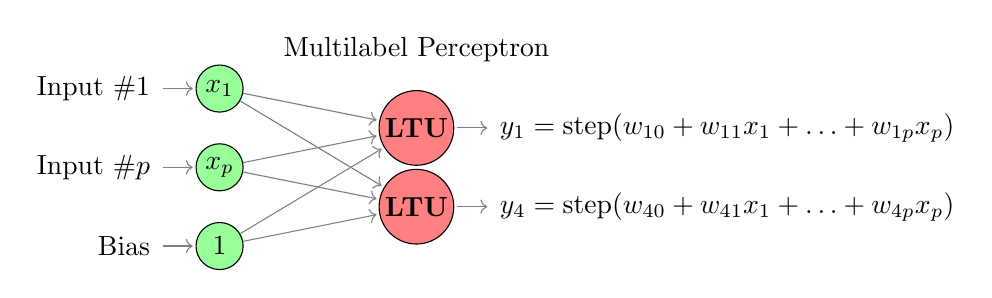
\begin{tikzpicture}[shorten >=1pt,->,draw=black!50, node distance=\layersep]
%https://tex.stackexchange.com/questions/96846/how-to-place-label-in-middle-of-line-above-and-below-with-tikz
    \tikzstyle{every pin edge}=[<-,shorten <=1pt]
    \tikzstyle{neuron}=[circle,fill=black!25,minimum size=17pt,inner sep=0pt, draw=black]
    \tikzstyle{input neuron}=[neuron, fill=green!40];
    \tikzstyle{output neuron}=[neuron, fill=red!50];
    \tikzstyle{hidden neuron}=[neuron, fill=blue!30];
    \tikzstyle{annot} = [text width=10em, text centered]

    % Draw the input layer nodes
	\node[input neuron, pin=left:Input \#1] (I-1) at (0,-1) {$x_1$};
	\node[input neuron, pin=left:Input \#$p$] (I-2) at (0,-2) {$x_p$};

    \node[input neuron, pin=left:Bias] (I-3) at (0,-3) {$1$};	
    % Draw the hidden layer nodes

        \node[output neuron, pin={[pin edge={->}]right: $y_1=\text{step}(w_{1 0}+w_{1 1}x_1+\ldots+ w_{1 p}x_p)$ }] (H-1) at (\layersep,- 1.5 cm) {$\,\textbf{LTU}\,$};
	 \node[output neuron, pin={[pin edge={->}]right: $y_4=\text{step}(w_{4 0}+w_{4 1}x_1+\ldots+ w_{4 p}x_p)$ }] (H-4) at (\layersep,- 2.5 cm) {$\,\textbf{LTU}\,$};

    \foreach \source in {1,...,3}
        \foreach \dest in {1,4}
		  \draw (I-\source) -- (H-\dest);

    \node[annot,above of=H-1, node distance=1cm] (hl) {Multilabel Perceptron};
\end{tikzpicture}
  \end{minipage}
  \vfill
\begin{minipage}[t][0.6\textheight][t]{\textwidth}
$$
\textbf{Learning Rule:}\hspace{1em} w_{ij}^{(n+1)} = w_{ij} + \eta(y_j-\hat y_j)x_i\,.
$$\pause
Pass a single training instance $x$ through the network:\pause

If the prediction on label $i$ is correct $\hat y_i = y_i$ and we do not update the weights $w_{ij}$. 

\pause If the prediction on label $i$ is incorrect, $\hat y_i\neq y_i$. So if the true labeling is $y_i = 1$, add $\eta x_i$ to all weights $w_{ij}$.\pause If $y_i = 0$, subtract $\eta x_i$ from all weights $w_{ij}$. \pause
\end{minipage}
\end{frame}







\begin{frame}[fragile]{Perceptron}
  \begin{minipage}[t][0.5\textheight][t]{\textwidth}
	\centering \includegraphics[height=0.5\textheight]{L11XORDist.png} 
  \end{minipage}
  \vfill
\begin{minipage}[t][0.5\textheight][t]{\textwidth}
The perceptron itself is one of the first examples of SGD, but it has some serious problems. In particular, it cannot solve some trivial problems like the xor labeling above. \pause

Although now unsurprising (no linear classifier can solve xor) the exceptions for the perceptron were high and when this problem was uncovered in 1969 it lead most researchers to abandon neural networks in favor of functional and logical methods.  
\end{minipage}
\end{frame}



\begin{frame}[fragile]{Perceptron}
  \begin{minipage}[t][0.4\textheight][t]{\textwidth}
\includegraphics[height=0.3\textheight]{L11XORDist2.png} \hspace{2em}
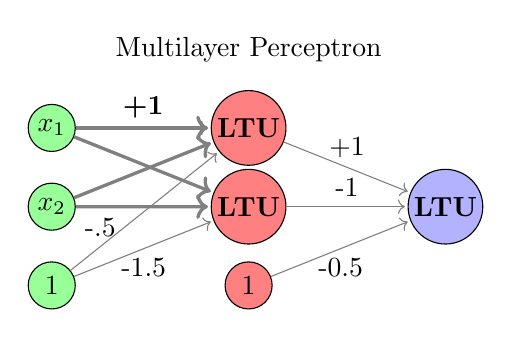
\begin{tikzpicture}[shorten >=1pt,->,draw=black!50, node distance=\layersep]
%https://tex.stackexchange.com/questions/96846/how-to-place-label-in-middle-of-line-above-and-below-with-tikz
    \tikzstyle{every pin edge}=[<-,shorten <=1pt]
    \tikzstyle{neuron}=[circle,fill=black!25,minimum size=17pt,inner sep=0pt, draw=black]
    \tikzstyle{input neuron}=[neuron, fill=green!40];
    \tikzstyle{output neuron}=[neuron, fill=red!50];
    \tikzstyle{hidden neuron}=[neuron, fill=blue!30];
    \tikzstyle{annot} = [text width=10em, text centered]

    % Draw the input layer nodes
	\node[input neuron] (I-1) at (0,-1) {$x_1$};
	\node[input neuron] (I-2) at (0,-2) {$x_2$};
      \node[input neuron] (I-3) at (0,-3) {$1$};	
    % Draw the hidden layer nodes

        \node[output neuron] (H-1) at (\layersep,-1 cm) {$\,\textbf{LTU}\,$};
	 \node[output neuron] (H-2) at (\layersep,- 2 cm) {$\,\textbf{LTU}\,$};
	 \node[output neuron] (H-3) at (\layersep,- 3 cm) {$\,1\,$};


	 \node[hidden neuron] (O-1) at (\layersep+\layersep,-2 cm) {$\,\textbf{LTU}\,$};

    \foreach \source in {1,...,2}
        \foreach \dest in {1,2}
		  \draw[very thick] (I-\source) -- (H-\dest);

	\draw (I-1) -- node[above, pos=0.5] {\textbf{+1}} ++ (H-1);	

	\draw (I-3) -- node[above, pos=0.2] {-.5} ++ (H-1);
	\draw (I-3) -- node[below, pos=0.5] {-1.5} ++ (H-2);

	\draw (H-1) -- node[above, pos=0.5] {+1} ++ (O-1);
	\draw (H-2) -- node[above, pos=0.5] {-1} ++ (O-1);
	\draw (H-3) -- node[below, pos=0.5] {-0.5} ++ (O-1);

    \node[annot,above of=H-1, node distance=1cm] (hl) {Multilayer Perceptron};
\end{tikzpicture}
  \end{minipage}
  \vfill
\begin{minipage}[t][0.6\textheight][t]{\textwidth}
However it was premature to abandon the perceptron: it turns out that if you stack perceptrons you can fit the xor distribution. \pause Consider sending the point $(0,0)$ through:
\begin{align*}
\action<+->{
{\color{green} (0,0)}\pause&\,\,\to \,\,  {\color{red} \text{step}(x_1+x_2-0.5,x_1+x_2-1.5) = (0,0)}
}
\\
\action<+->{
&\,\,\to \,\,  {\color{blue} \text{step}[(0)-(0)+(-0.5)] = 0}
}
\end{align*}
\end{minipage}
\end{frame}


\begin{frame}[fragile]{Perceptron}
  \begin{minipage}[t][0.4\textheight][t]{\textwidth}
\includegraphics[height=0.3\textheight]{L11XORDist2.png} \hspace{2em}
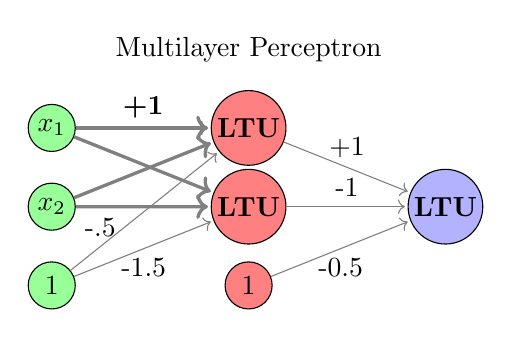
\begin{tikzpicture}[shorten >=1pt,->,draw=black!50, node distance=\layersep]
%https://tex.stackexchange.com/questions/96846/how-to-place-label-in-middle-of-line-above-and-below-with-tikz
    \tikzstyle{every pin edge}=[<-,shorten <=1pt]
    \tikzstyle{neuron}=[circle,fill=black!25,minimum size=17pt,inner sep=0pt, draw=black]
    \tikzstyle{input neuron}=[neuron, fill=green!40];
    \tikzstyle{output neuron}=[neuron, fill=red!50];
    \tikzstyle{hidden neuron}=[neuron, fill=blue!30];
    \tikzstyle{annot} = [text width=10em, text centered]

    % Draw the input layer nodes
	\node[input neuron] (I-1) at (0,-1) {$x_1$};
	\node[input neuron] (I-2) at (0,-2) {$x_2$};
      \node[input neuron] (I-3) at (0,-3) {$1$};	
    % Draw the hidden layer nodes

        \node[output neuron] (H-1) at (\layersep,-1 cm) {$\,\textbf{LTU}\,$};
	 \node[output neuron] (H-2) at (\layersep,- 2 cm) {$\,\textbf{LTU}\,$};
	 \node[output neuron] (H-3) at (\layersep,- 3 cm) {$\,1\,$};


	 \node[hidden neuron] (O-1) at (\layersep+\layersep,-2 cm) {$\,\textbf{LTU}\,$};

    \foreach \source in {1,...,2}
        \foreach \dest in {1,2}
		  \draw[very thick] (I-\source) -- (H-\dest);

	\draw (I-1) -- node[above, pos=0.5] {\textbf{+1}} ++ (H-1);	

	\draw (I-3) -- node[above, pos=0.2] {-.5} ++ (H-1);
	\draw (I-3) -- node[below, pos=0.5] {-1.5} ++ (H-2);

	\draw (H-1) -- node[above, pos=0.5] {+1} ++ (O-1);
	\draw (H-2) -- node[above, pos=0.5] {-1} ++ (O-1);
	\draw (H-3) -- node[below, pos=0.5] {-0.5} ++ (O-1);

    \node[annot,above of=H-1, node distance=1cm] (hl) {Multilayer Perceptron};
\end{tikzpicture}
  \end{minipage}
  \vfill
\begin{minipage}[t][0.6\textheight][t]{\textwidth}
Sending (1,1) through, we get
\begin{align*}
\action<+->{
{\color{green} (1,1)}\pause&\,\,\to \,\,  {\color{red} \text{step}(1+1-0.5,1+1-1.5) = (1,1)}
}
\\
\action<+->{
&\,\,\to \,\,  {\color{blue} \text{step}[(1)-(1)+(-0.5)] = 0}
}
\end{align*}
\action<+->{(\textbf{Exercise:}) Verify that (0,1) and (1,0) are labeled 1.}
\end{minipage}
\end{frame}



\begin{frame}[fragile]{Perceptron}
  \begin{minipage}[t][0.4\textheight][t]{\textwidth}
\includegraphics[height=0.3\textheight]{L11XORDist2.png} \hspace{2em}
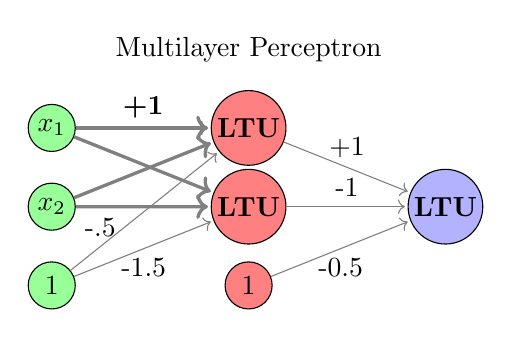
\begin{tikzpicture}[shorten >=1pt,->,draw=black!50, node distance=\layersep]
%https://tex.stackexchange.com/questions/96846/how-to-place-label-in-middle-of-line-above-and-below-with-tikz
    \tikzstyle{every pin edge}=[<-,shorten <=1pt]
    \tikzstyle{neuron}=[circle,fill=black!25,minimum size=17pt,inner sep=0pt, draw=black]
    \tikzstyle{input neuron}=[neuron, fill=green!40];
    \tikzstyle{output neuron}=[neuron, fill=red!50];
    \tikzstyle{hidden neuron}=[neuron, fill=blue!30];
    \tikzstyle{annot} = [text width=10em, text centered]

    % Draw the input layer nodes
	\node[input neuron] (I-1) at (0,-1) {$x_1$};
	\node[input neuron] (I-2) at (0,-2) {$x_2$};
      \node[input neuron] (I-3) at (0,-3) {$1$};	
    % Draw the hidden layer nodes

        \node[output neuron] (H-1) at (\layersep,-1 cm) {$\,\textbf{LTU}\,$};
	 \node[output neuron] (H-2) at (\layersep,- 2 cm) {$\,\textbf{LTU}\,$};
	 \node[output neuron] (H-3) at (\layersep,- 3 cm) {$\,1\,$};


	 \node[hidden neuron] (O-1) at (\layersep+\layersep,-2 cm) {$\,\textbf{LTU}\,$};

    \foreach \source in {1,...,2}
        \foreach \dest in {1,2}
		  \draw[very thick] (I-\source) -- (H-\dest);

	\draw (I-1) -- node[above, pos=0.5] {\textbf{+1}} ++ (H-1);	

	\draw (I-3) -- node[above, pos=0.2] {-.5} ++ (H-1);
	\draw (I-3) -- node[below, pos=0.5] {-1.5} ++ (H-2);

	\draw (H-1) -- node[above, pos=0.5] {+1} ++ (O-1);
	\draw (H-2) -- node[above, pos=0.5] {-1} ++ (O-1);
	\draw (H-3) -- node[below, pos=0.5] {-0.5} ++ (O-1);

    \node[annot,above of=H-1, node distance=1cm] (hl) {Multilayer Perceptron};
\end{tikzpicture}
  \end{minipage}
  \vfill
\begin{minipage}[t][0.6\textheight][t]{\textwidth}
With a little bit of work, one can show that this multilayer perceptron actually is the fitting on the left:
$$
\hat{h}(x_1,x_2) = \begin{cases}
1 &0.5 - x_1 \leq x_2 \leq 1.5 - x_1
\\
0 &\text{otherwise}
\end{cases}
$$
\textbf{Questions:} What is the hypothesis class of all two layer two variable perceptrons? How would we construct a perceptron with three linear conditions?
\end{minipage}
\end{frame}




\section{Gradient Decent and Back Propagation}





\begin{frame}[fragile]{Training the Multilayer Perceptron}
\begin{minipage}[t][0.5\textheight][t]{\textwidth}\centering
\begin{tikzpicture}[shorten >=1pt,->,draw=black!50, node distance=\layersep]
%https://tex.stackexchange.com/questions/96846/how-to-place-label-in-middle-of-line-above-and-below-with-tikz
    \tikzstyle{every pin edge}=[<-,shorten <=1pt]
    \tikzstyle{neuron}=[circle,fill=black!25,minimum size=17pt,inner sep=0pt, draw=black]
    \tikzstyle{input neuron}=[neuron, fill=green!50];
    \tikzstyle{output neuron}=[neuron, fill=red!50];
    \tikzstyle{hidden neuron}=[neuron, fill=blue!30];
    \tikzstyle{annot} = [text width=4em, text centered]

    % Draw the input layer nodes
    \foreach \name / \y in {1,...,3}
    % This is the same as writing \foreach \name / \y in {1/1,2/2,3/3,4/4}
        \node[input neuron] (I-\name) at (0,-\y) {$x_\y$};

    % Draw the hidden layer nodes
    \foreach \name / \y in {1,...,3}
        \path[yshift=0cm]
            node[hidden neuron] (H1-\name) at (\layersep,-\y cm) {$\, LTU\, $};

    % Draw the hidden layer nodes
    \foreach \name / \y in {1,...,3}
        \path[yshift=0cm]
            node[hidden neuron] (H2-\name) at (\layersep + \layersep,-\y cm) {$\, LTU\, $};


    % Draw the output layer node
    \foreach \name / \y in {1,...,2}
    		\node[output neuron,pin={[pin edge={->}]right:Output}] (O-\y) at (\layersep + \layersep + \layersep,-\y cm-.5cm) {$\,LTU\,$};

    % Connect every node in the input layer with every node in the
    % hidden layer.
    \foreach \source in {1,...,3}
        \foreach \dest in {1,...,3}
            \draw (I-\source) --  (H1-\dest);

    % Connect every node in the input layer with every node in the
    % hidden layer.
    \foreach \source in {1,...,3}
        \foreach \dest in {1,...,3}
            \draw (H1-\source) --  (H2-\dest);


    % Connect every node in the hidden layer with the output layer
    \foreach \source in {1,...,3}
		\foreach \dest in {1,...,2}
        		\path (H2-\source) edge (O-\dest);

    % Annotate the layers
    \node[annot,above of=H-1, node distance=1cm] (hl) {Hidden layer};
    \node[annot,left of=hl] {Input layer};
    \node[annot,right of=hl] (hl2) {Hidden layer};
    \node[annot,right of=hl2] {Output layer};
\end{tikzpicture}
  \end{minipage}
  \vfill
\begin{minipage}[t][0.5\textheight][t]{\textwidth}
A multilayer perceptron (MLP) is composed of one input layer, multiple hidden layers and an output layer. If the network has more than one hidden layer it is called a \textbf{deep neural network}.\newline

For a deep network, each layer represents a linear combination of the previous layers, with each output composed by an activation function.  
\end{minipage}
\end{frame}





\begin{frame}[fragile]{Training the Multilayer Perceptron}
\begin{minipage}[t][0.5\textheight][t]{\textwidth}\centering
\begin{tikzpicture}[shorten >=1pt,->,draw=black!50, node distance=\layersep]
%https://tex.stackexchange.com/questions/96846/how-to-place-label-in-middle-of-line-above-and-below-with-tikz
    \tikzstyle{every pin edge}=[<-,shorten <=1pt]
    \tikzstyle{neuron}=[circle,fill=black!25,minimum size=17pt,inner sep=0pt, draw=black]
    \tikzstyle{input neuron}=[neuron, fill=green!50];
    \tikzstyle{output neuron}=[neuron, fill=red!50];
    \tikzstyle{hidden neuron}=[neuron, fill=blue!30];
    \tikzstyle{annot} = [text width=4em, text centered]

    % Draw the input layer nodes
    \foreach \name / \y in {1,...,3}
    % This is the same as writing \foreach \name / \y in {1/1,2/2,3/3,4/4}
        \node[input neuron] (I-\name) at (0,-\y) {$x_\y$};

    % Draw the hidden layer nodes
    \foreach \name / \y in {1,...,3}
        \path[yshift=0cm]
            node[hidden neuron] (H1-\name) at (\layersep,-\y cm) {$\, LTU\, $};

    % Draw the hidden layer nodes
    \foreach \name / \y in {1,...,3}
        \path[yshift=0cm]
            node[hidden neuron] (H2-\name) at (\layersep + \layersep,-\y cm) {$\, LTU\, $};


    % Draw the output layer node
    \foreach \name / \y in {1,...,2}
    		\node[output neuron,pin={[pin edge={->}]right:Output}] (O-\y) at (\layersep + \layersep + \layersep,-\y cm-.5cm) {$\,LTU\,$};

    % Connect every node in the input layer with every node in the
    % hidden layer.
    \foreach \source in {1,...,3}
        \foreach \dest in {1,...,3}
            \draw (I-\source) --  (H1-\dest);

    % Connect every node in the input layer with every node in the
    % hidden layer.
    \foreach \source in {1,...,3}
        \foreach \dest in {1,...,3}
            \draw (H1-\source) --  (H2-\dest);


    % Connect every node in the hidden layer with the output layer
    \foreach \source in {1,...,3}
		\foreach \dest in {1,...,2}
        		\path (H2-\source) edge (O-\dest);

    % Annotate the layers
    \node[annot,above of=H-1, node distance=1cm] (hl) {Hidden layer};
    \node[annot,left of=hl] {Input layer};
    \node[annot,right of=hl] (hl2) {Hidden layer};
    \node[annot,right of=hl2] {Output layer};
\end{tikzpicture}
  \end{minipage}
  \vfill
\begin{minipage}[t][0.5\textheight][t]{\textwidth}
For the $j$'th hidden layer, let $N^{j}$ be a column vector of $n_j$ nodes $N_{k}^j$. Let $\sigma$ be an activation function applied component-wise and let $W_{\ell k}^j$ be outgoing weights.  The values of the nodes in the $j+1$'st layer will be
$$
N^{j+1} = \sigma\left(\, W^{j}N^{j} \,\right)\,.
$$
Here, $W^j$ is a $n_j\times n_{j+1}$ matrix. 
\end{minipage}
\end{frame}







\begin{frame}[fragile]{Training the Multilayer Perceptron}
\begin{minipage}[t][0.5\textheight][t]{\textwidth}\centering
\begin{tikzpicture}[shorten >=1pt,->,draw=black!50, node distance=\layersep]
%https://tex.stackexchange.com/questions/96846/how-to-place-label-in-middle-of-line-above-and-below-with-tikz
    \tikzstyle{every pin edge}=[<-,shorten <=1pt]
    \tikzstyle{neuron}=[circle,fill=black!25,minimum size=17pt,inner sep=0pt, draw=black]
    \tikzstyle{input neuron}=[neuron, fill=green!50];
    \tikzstyle{output neuron}=[neuron, fill=red!50];
    \tikzstyle{hidden neuron}=[neuron, fill=blue!30];
    \tikzstyle{annot} = [text width=4em, text centered]

    % Draw the input layer nodes
    \foreach \name / \y in {1,...,3}
    % This is the same as writing \foreach \name / \y in {1/1,2/2,3/3,4/4}
        \node[input neuron] (I-\name) at (0,-\y) {$x_\y$};

    % Draw the hidden layer nodes
    \foreach \name / \y in {1,...,3}
        \path[yshift=0cm]
            node[hidden neuron] (H1-\name) at (\layersep,-\y cm) {$\, LTU\, $};

    % Draw the hidden layer nodes
    \foreach \name / \y in {1,...,3}
        \path[yshift=0cm]
            node[hidden neuron] (H2-\name) at (\layersep + \layersep,-\y cm) {$\, LTU\, $};


    % Draw the output layer node
    \foreach \name / \y in {1,...,2}
    		\node[output neuron,pin={[pin edge={->}]right:Output}] (O-\y) at (\layersep + \layersep + \layersep,-\y cm-.5cm) {$\,LTU\,$};

    % Connect every node in the input layer with every node in the
    % hidden layer.
    \foreach \source in {1,...,3}
        \foreach \dest in {1,...,3}
            \draw (I-\source) --  (H1-\dest);

    % Connect every node in the input layer with every node in the
    % hidden layer.
    \foreach \source in {1,...,3}
        \foreach \dest in {1,...,3}
            \draw (H1-\source) --  (H2-\dest);


    % Connect every node in the hidden layer with the output layer
    \foreach \source in {1,...,3}
		\foreach \dest in {1,...,2}
        		\path (H2-\source) edge (O-\dest);

    % Annotate the layers
    \node[annot,above of=H-1, node distance=1cm] (hl) {Hidden layer};
    \node[annot,left of=hl] {Input layer};
    \node[annot,right of=hl] (hl2) {Hidden layer};
    \node[annot,right of=hl2] {Output layer};
\end{tikzpicture}
  \end{minipage}
  \vfill
\begin{minipage}[t][0.5\textheight][t]{\textwidth}
If the input is $X$ and the output is $Y$, the whole $L$ layer network is a function 
$$
F(X) = \sigma\left(\, W^{L-1} \sigma( \,W^{L-2}\ldots \sigma(W^0 X)\ldots) \, \right)\,.
$$
Here, $W^j$ is a $n_k\times n_{k+1}$ matrix. 
\end{minipage}
\end{frame}






\begin{frame}[fragile]{Training the Multilayer Perceptron}
\begin{minipage}[t][0.5\textheight][t]{\textwidth}\centering
\begin{tikzpicture}[shorten >=1pt,->,draw=black!50, node distance=\layersep]
%https://tex.stackexchange.com/questions/96846/how-to-place-label-in-middle-of-line-above-and-below-with-tikz
    \tikzstyle{every pin edge}=[<-,shorten <=1pt]
    \tikzstyle{neuron}=[circle,fill=black!25,minimum size=17pt,inner sep=0pt, draw=black]
    \tikzstyle{input neuron}=[neuron, fill=green!50];
    \tikzstyle{output neuron}=[neuron, fill=red!50];
    \tikzstyle{hidden neuron}=[neuron, fill=blue!30];
    \tikzstyle{annot} = [text width=4em, text centered]

    % Draw the input layer nodes
    \foreach \name / \y in {1,...,3}
    % This is the same as writing \foreach \name / \y in {1/1,2/2,3/3,4/4}
        \node[input neuron] (I-\name) at (0,-\y) {$x_\y$};

    % Draw the hidden layer nodes
    \foreach \name / \y in {1,...,3}
        \path[yshift=0cm]
            node[hidden neuron] (H1-\name) at (\layersep,-\y cm) {$\, LTU\, $};

    % Draw the hidden layer nodes
    \foreach \name / \y in {1,...,3}
        \path[yshift=0cm]
            node[hidden neuron] (H2-\name) at (\layersep + \layersep,-\y cm) {$\, LTU\, $};


    % Draw the output layer node
    \foreach \name / \y in {1,...,2}
    		\node[output neuron,pin={[pin edge={->}]right:Output}] (O-\y) at (\layersep + \layersep + \layersep,-\y cm-.5cm) {$\,LTU\,$};

    % Connect every node in the input layer with every node in the
    % hidden layer.
    \foreach \source in {1,...,3}
        \foreach \dest in {1,...,3}
            \draw (I-\source) --  (H1-\dest);

    % Connect every node in the input layer with every node in the
    % hidden layer.
    \foreach \source in {1,...,3}
        \foreach \dest in {1,...,3}
            \draw (H1-\source) --  (H2-\dest);


    % Connect every node in the hidden layer with the output layer
    \foreach \source in {1,...,3}
		\foreach \dest in {1,...,2}
        		\path (H2-\source) edge (O-\dest);

    % Annotate the layers
    \node[annot,above of=H-1, node distance=1cm] (hl) {Hidden layer};
    \node[annot,left of=hl] {Input layer};
    \node[annot,right of=hl] (hl2) {Hidden layer};
    \node[annot,right of=hl2] {Output layer};
\end{tikzpicture}
  \end{minipage}
  \vfill
\begin{minipage}[t][0.5\textheight][t]{\textwidth}
It's clear that the number of weights in a network becomes large \emph{fast}:
$$
\text{\# Weights:} \hspace{2em} |w| = (n_{K}\times n{L-1}^2\ldots, n_1^2\times n_0\,.
$$
Learning how to effectively train MLP took another 20 years. 
\end{minipage}
\end{frame}





\begin{frame}[fragile]{Training the Multilayer Perceptron}
\begin{minipage}[t][0.5\textheight][t]{\textwidth}\centering
\begin{tikzpicture}[shorten >=1pt,->,draw=black!50, node distance=\layersep]
%https://tex.stackexchange.com/questions/96846/how-to-place-label-in-middle-of-line-above-and-below-with-tikz
    \tikzstyle{every pin edge}=[<-,shorten <=1pt]
    \tikzstyle{neuron}=[circle,fill=black!25,minimum size=17pt,inner sep=0pt, draw=black]
    \tikzstyle{input neuron}=[neuron, fill=green!50];
    \tikzstyle{output neuron}=[neuron, fill=red!50];
    \tikzstyle{hidden neuron}=[neuron, fill=blue!30];
    \tikzstyle{annot} = [text width=4em, text centered]

    % Draw the input layer nodes
    \foreach \name / \y in {1,...,3}
    % This is the same as writing \foreach \name / \y in {1/1,2/2,3/3,4/4}
        \node[input neuron] (I-\name) at (0,-\y) {$x_\y$};

    % Draw the hidden layer nodes
    \foreach \name / \y in {1,...,3}
        \path[yshift=0cm]
            node[hidden neuron] (H1-\name) at (\layersep,-\y cm) {$\, LTU\, $};

    % Draw the hidden layer nodes
    \foreach \name / \y in {1,...,3}
        \path[yshift=0cm]
            node[hidden neuron] (H2-\name) at (\layersep + \layersep,-\y cm) {$\, LTU\, $};


    % Draw the output layer node
    \foreach \name / \y in {1,...,2}
    		\node[output neuron,pin={[pin edge={->}]right:Output}] (O-\y) at (\layersep + \layersep + \layersep,-\y cm-.5cm) {$\,LTU\,$};

    % Connect every node in the input layer with every node in the
    % hidden layer.
    \foreach \source in {1,...,3}
        \foreach \dest in {1,...,3}
            \draw (I-\source) --  (H1-\dest);

    % Connect every node in the input layer with every node in the
    % hidden layer.
    \foreach \source in {1,...,3}
        \foreach \dest in {1,...,3}
            \draw (H1-\source) --  (H2-\dest);


    % Connect every node in the hidden layer with the output layer
    \foreach \source in {1,...,3}
		\foreach \dest in {1,...,2}
        		\path (H2-\source) edge (O-\dest);

    % Annotate the layers
    \node[annot,above of=H-1, node distance=1cm] (hl) {Hidden layer};
    \node[annot,left of=hl] {Input layer};
    \node[annot,right of=hl] (hl2) {Hidden layer};
    \node[annot,right of=hl2] {Output layer};
\end{tikzpicture}
  \end{minipage}
  \vfill
\begin{minipage}[t][0.5\textheight][t]{\textwidth}
The problem with training wasn't just a large number of constants, but fact that the step function has 0 gradient everywhere, so there is no indication of which direction to move. 

To compute the gradient the activation function for the LSU was replaced by the \textbf{logistic} or \textbf{sigmoid} function 
$$
\sigma(z) = \frac{1}{1-e^{-x}}\,.
$$
\end{minipage}
\end{frame}




\begin{frame}[fragile]{Implementing Gradient Decent}
  \begin{minipage}[t][0.5\textheight][t]{\textwidth}
	\centering \includegraphics[width=0.9\textwidth]{L11LossFunctions3.png} 
  \end{minipage}
  \vfill
\begin{minipage}[t][0.5\textheight][t]{\textwidth}

Other popular alternatives to the step function are 
$$
\tanh(x) = 2\sigma(2x) - 1
$$
and 
$$
\text{ReLU}(x) = \max\{0,x\} = (x)_+
$$
\end{minipage}
\end{frame}






\begin{frame}[fragile]{Training the Multilayer Perceptron}
\begin{minipage}[t][0.5\textheight][t]{\textwidth}\centering
\begin{tikzpicture}[shorten >=1pt,->,draw=black!50, node distance=\layersep]
%https://tex.stackexchange.com/questions/96846/how-to-place-label-in-middle-of-line-above-and-below-with-tikz
    \tikzstyle{every pin edge}=[<-,shorten <=1pt]
    \tikzstyle{neuron}=[circle,fill=black!25,minimum size=17pt,inner sep=0pt, draw=black]
    \tikzstyle{input neuron}=[neuron, fill=green!50];
    \tikzstyle{output neuron}=[neuron, fill=red!50];
    \tikzstyle{hidden neuron}=[neuron, fill=blue!30];
    \tikzstyle{annot} = [text width=4em, text centered]

    % Draw the input layer nodes
    \foreach \name / \y in {1,...,3}
    % This is the same as writing \foreach \name / \y in {1/1,2/2,3/3,4/4}
        \node[input neuron] (I-\name) at (0,-\y) {$x_\y$};

    % Draw the hidden layer nodes
    \foreach \name / \y in {1,...,3}
        \path[yshift=0cm]
            node[hidden neuron] (H1-\name) at (\layersep,-\y cm) {$\, LTU\, $};

    % Draw the hidden layer nodes
    \foreach \name / \y in {1,...,3}
        \path[yshift=0cm]
            node[hidden neuron] (H2-\name) at (\layersep + \layersep,-\y cm) {$\, LTU\, $};


    % Draw the output layer node
    \foreach \name / \y in {1,...,2}
    		\node[output neuron,pin={[pin edge={->}]right:Output}] (O-\y) at (\layersep + \layersep + \layersep,-\y cm-.5cm) {$\,LTU\,$};

    % Connect every node in the input layer with every node in the
    % hidden layer.
    \foreach \source in {1,...,3}
        \foreach \dest in {1,...,3}
            \draw (I-\source) --  (H1-\dest);

    % Connect every node in the input layer with every node in the
    % hidden layer.
    \foreach \source in {1,...,3}
        \foreach \dest in {1,...,3}
            \draw (H1-\source) --  (H2-\dest);


    % Connect every node in the hidden layer with the output layer
    \foreach \source in {1,...,3}
		\foreach \dest in {1,...,2}
        		\path (H2-\source) edge (O-\dest);

    % Annotate the layers
    \node[annot,above of=H-1, node distance=1cm] (hl) {Hidden layer};
    \node[annot,left of=hl] {Input layer};
    \node[annot,right of=hl] (hl2) {Hidden layer};
    \node[annot,right of=hl2] {Output layer};
\end{tikzpicture}
  \end{minipage}
  \vfill
\begin{minipage}[t][0.5\textheight][t]{\textwidth}
In 1986, D. E. Rumelhart popularized the idea of \textbf{back propagation} to estimate gradients. Although back propagation is the most widely used today, we will first canvas the common methods of gradient estimation. 
\end{minipage}
\end{frame}








\begin{frame}[fragile]{Implementing Gradient Decent}
There are several popular ways of implementing gradient decent. For a loss function like MSE, gradient decent updates the parameters at each step by
$$
\beta^{(n+1)} = \beta^{(n)} - \eta \nabla_{\beta} \text{MSE}(\beta^{(n)}).
$$\pause
If there is a closed form formula for MSE, the update step can be computed explicitly. This is known as \textbf{manual differentiation} or \textbf{pen and paper differentiation}. \pause

If the nodes are fairly out of the box, we can try to use automatic \textbf{symbolic differentiation} to pass through the graph and create a gradient. There are some decent solvers out there and this is an active area of development, but unfortunately it often yields huge redundant computations that allow errors to propagate. It is also must be implemented manually on arbitrary code.
\end{frame}



\begin{frame}[fragile]{Numerical Differential }
Numerical differentiation is the simplest general solver. For a network $Y = h_\beta(X)$ with inputs $X$ and outputs $Y$ we implement partial differentiation by passing a data point (or points) through the network and seeing how a small change in $\beta$ effects it
$$
\frac{\partial h_\beta}{\partial \beta} \approx \frac{1}{N}\sum_{i=1}^N\frac{h_{\beta+\epsilon}(X_i) - h_{\beta}(X_i) }{\epsilon}\,, \hspace{2em} \epsilon\ll 1\,.
$$\pause
For a large network, this takes many calls to the function while also being numerically suspect. It is however a good first pass test and it is easy to implement. 
\end{frame}



\begin{frame}[fragile]{Autodiff}
\textbf{Forward mode autodiff} is a mixture of numerical and symbolic differentiation. It relies on \textbf{dual numbers} (\textbf{infinitesimals} in the math context), that is we write
$$
a+b\epsilon
$$
where $\epsilon$ is "small," ie $\epsilon^2 = 0$. In memory, dual numbers are stored as a pair of floats $(a,b)$. \pause

Dual numbers have slightly nonstandard multiplication and exponentiation that encode the rules of differentiation implicitly:
$$
(a+b\epsilon)(c+d\epsilon) = ac+(bc+ad)\epsilon\,,\hspace{2em} e^{a+b\epsilon} = e^a(1+b\epsilon)\,.
$$
Both equations are derive by expanding $e^{b\epsilon}$ and using $\epsilon^2$ and higher order terms to 0. \pause In fact, if $f(x)$ is smooth than by Taylors theorem
$$
f(a+b\epsilon) = f(a)+b\epsilon f'(a)\,.
$$
\end{frame}




\begin{frame}[fragile]{Forward Autodiff}
  \begin{minipage}[t][0.5\textheight][t]{\textwidth}
	\centering
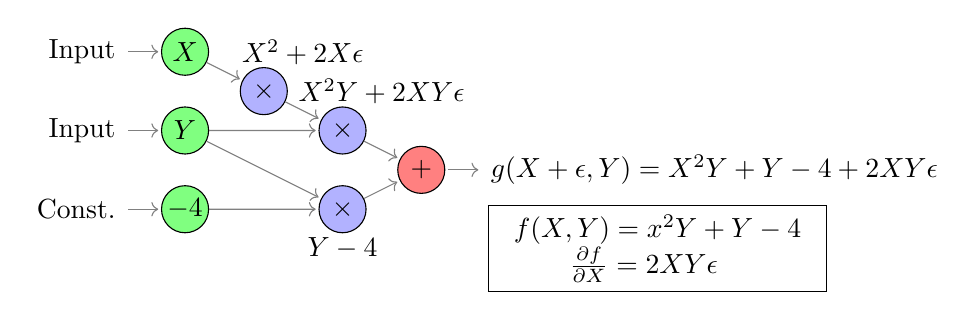
\begin{tikzpicture}[shorten >=1pt,->,draw=black!50, node distance=\layersep]
%https://tex.stackexchange.com/questions/96846/how-to-place-label-in-middle-of-line-above-and-below-with-tikz
    \tikzstyle{every pin edge}=[<-,shorten <=1pt]
    \tikzstyle{neuron}=[circle,fill=black!25,minimum size=17pt,inner sep=0pt, draw=black]
    \tikzstyle{input neuron}=[neuron, fill=green!50];
    \tikzstyle{output neuron}=[neuron, fill=red!50];
    \tikzstyle{hidden neuron}=[neuron, fill=blue!30];
    \tikzstyle{annot} = [text width=4em, text centered]


    \node[input neuron, pin=left:Input] (I-1) at (0,-1) {$X$};
    \node[input neuron, pin=left:Input] (I-2) at (0,-2) {$Y$};
    \node[input neuron, pin=left:Const.] (I-3) at (0,-3) {$-4$};

    \node[hidden neuron] (H1-1) at (1cm,-1.5 cm) {$\times$};

    \node[hidden neuron] (H2-1) at (2cm,-2 cm) {$\times$};
    \node[hidden neuron] (H2-2) at (2cm,-3 cm) {$\times$};

    \node[output neuron,pin={[pin edge={->}]right:$g(X+\epsilon,Y) = X^2Y+Y-4 + 2XY\epsilon$}] (O) at (3cm,-2.5 cm) {$+$};
    \draw (I-1) -- (H1-1);
    \draw (H1-1) -- (H2-1);
    \draw (I-2) -- (H2-1);
    \draw (H2-1) -- (O);
    \draw (I-2) -- (H2-2);
    \draw (I-3) -- (H2-2);
    \draw (H2-2) -- (O);

	\node[above right of=H1-1, node distance=.7cm] {$X^2+2X\epsilon$};
	\node[above right of=H2-1, node distance=.7cm] {$X^2Y+2XY\epsilon$};
	\node[below of=H2-2, node distance=.5cm] {$Y-4$};

    \node[] (T) at (6cm,-3.5 cm) {\boxed{\begin{tabular}{c}$f(X,Y) = x^2Y + Y-4$\\ $\frac{\partial f}{\partial X} = 2XY\epsilon \hspace{1em}$ \end{tabular}}};

\end{tikzpicture}
  \end{minipage}
  \vfill
\begin{minipage}[t][0.5\textheight][t]{\textwidth}
Since $f(a+b\epsilon) = f(a)+b\epsilon f'(a)$ gives you both $f(a)$ and $f'(a)$ in one go, implementing forward autodiff comes down to creating a new graph that computes the result of passing the dual number through the graph.\newline\pause

Of course, we intend to differentiate with respect to the weights, but that is equivalent to treating the weights as dual numbers.
\end{minipage}
\end{frame}











\begin{frame}[fragile]{Reverse Autodiff}
  \begin{minipage}[t][0.5\textheight][t]{\textwidth}
	\centering 
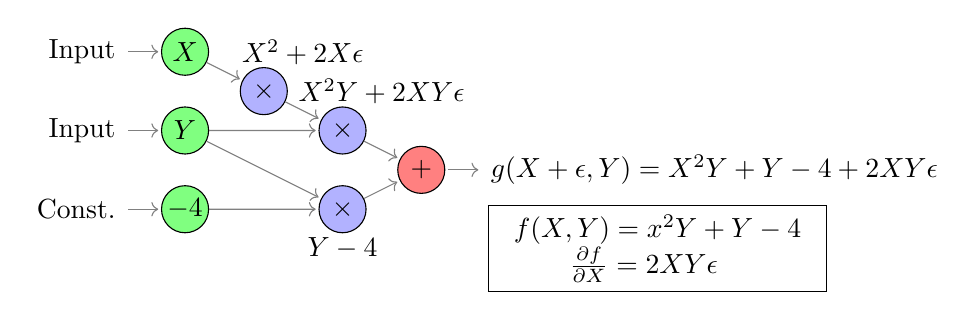
\begin{tikzpicture}[shorten >=1pt,->,draw=black!50, node distance=\layersep]
%https://tex.stackexchange.com/questions/96846/how-to-place-label-in-middle-of-line-above-and-below-with-tikz
    \tikzstyle{every pin edge}=[<-,shorten <=1pt]
    \tikzstyle{neuron}=[circle,fill=black!25,minimum size=17pt,inner sep=0pt, draw=black]
    \tikzstyle{input neuron}=[neuron, fill=green!50];
    \tikzstyle{output neuron}=[neuron, fill=red!50];
    \tikzstyle{hidden neuron}=[neuron, fill=blue!30];
    \tikzstyle{annot} = [text width=4em, text centered]


    \node[input neuron, pin=left:Input] (I-1) at (0,-1) {$X$};
    \node[input neuron, pin=left:Input] (I-2) at (0,-2) {$Y$};
    \node[input neuron, pin=left:Const.] (I-3) at (0,-3) {$-4$};

    \node[hidden neuron] (H1-1) at (1cm,-1.5 cm) {$\times$};

    \node[hidden neuron] (H2-1) at (2cm,-2 cm) {$\times$};
    \node[hidden neuron] (H2-2) at (2cm,-3 cm) {$\times$};

    \node[output neuron,pin={[pin edge={->}]right:$g(X+\epsilon,Y) = X^2Y+Y-4 + 2XY\epsilon$}] (O) at (3cm,-2.5 cm) {$+$};
    \draw (I-1) -- (H1-1);
    \draw (H1-1) -- (H2-1);
    \draw (I-2) -- (H2-1);
    \draw (H2-1) -- (O);
    \draw (I-2) -- (H2-2);
    \draw (I-3) -- (H2-2);
    \draw (H2-2) -- (O);

	\node[above right of=H1-1, node distance=.7cm] {$X^2+2X\epsilon$};
	\node[above right of=H2-1, node distance=.7cm] {$X^2Y+2XY\epsilon$};
	\node[below of=H2-2, node distance=.5cm] {$Y-4$};

    \node[] (T) at (6cm,-3.5 cm) {\boxed{\begin{tabular}{c}$f(X,Y) = x^2Y + Y-4$\\ $\frac{\partial f}{\partial X} = 2XY\epsilon \hspace{1em}$ \end{tabular}}};

\end{tikzpicture}
  \end{minipage}
  \vfill
\begin{minipage}[t][0.5\textheight][t]{\textwidth}
Forward autodiff is exact (unlike numerical approximation) but it still involves passing through the graph once for each weight $\beta$. For a graph with many connection weights this cause take a long time. \textbf{Reverse autodiff}, or \textbf{back propagation} on the other hand passes through the graph exactly twice.
\end{minipage}
\end{frame}


\section{Back Propagation}


\begin{frame}[fragile]{Reverse Autodiff}

\textbf{Reverse autodiff} constructs a new graph containing the derivative of each input node with respect to each output node. It then uses the chain rule
$$
\frac{\partial f}{\partial x} = \frac{\partial f}{\partial n} \frac{\partial n}{\partial x} 
$$
to compute the derivative by filling out a dual graph one step at a time. 

\textbf{Back propagation} uses reverse auto differentiation to compute the gradient for a fixed input-output pair $(x_i,y_i)$. The speed increase comes from the fact that computing $\frac{\partial F}{\partial w}$ for each weight requires many redundant calculations. By keeping track of these, and computing the chain rule in a reverse layer by layer fashion, we are able to compute the gradient via an adjoint network  graph. 
\end{frame}







\begin{frame}[fragile]{Reverse Autodiff}
  \begin{minipage}[t][0.5\textheight][t]{\textwidth}\centering
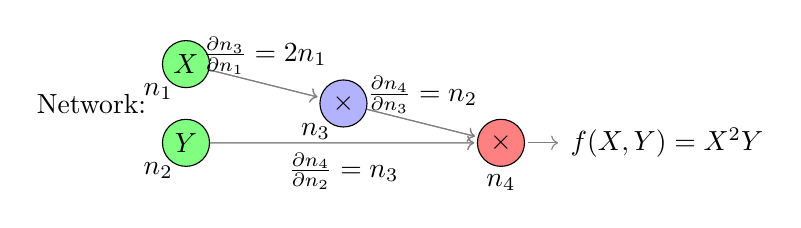
\begin{tikzpicture}[shorten >=1pt,->,draw=black!50, node distance=\layersep]
%https://tex.stackexchange.com/questions/96846/how-to-place-label-in-middle-of-line-above-and-below-with-tikz
    \tikzstyle{every pin edge}=[<-,shorten <=1pt]
    \tikzstyle{neuron}=[circle,fill=black!25,minimum size=17pt,inner sep=0pt, draw=black]
    \tikzstyle{input neuron}=[neuron, fill=green!50];
    \tikzstyle{output neuron}=[neuron, fill=red!50];
    \tikzstyle{hidden neuron}=[neuron, fill=blue!30];
    \tikzstyle{annot} = [text width=4em, text centered]


    \node[input neuron] (I-1) at (0,-1) {$X$};
    \node[input neuron] (I-2) at (0,-2) {$Y$};

    \node[hidden neuron] (H) at (2cm,-1.5 cm) {$\times$};

    \node[output neuron,pin={[pin edge={->}]right:$f(X,Y) = X^2Y$}] (O) at (4cm,-2 cm) {$\times$};
    \draw (I-1) -- (H);
    \draw (H) -- (O);
    \draw (I-2) -- (O);

	\node[below left of=I-1, node distance=.5cm] {$n_1$};
	\node[below left of=I-2, node distance=.5cm] {$n_2$};
	\node[below left of=H, node distance=.5cm] {$n_3$};
	\node[below of=O, node distance=.5cm] {$n_4$};

	\node[] at (-1.2cm,-1.5cm) {Network:};

    \draw (I-1) -- node[above, pos=0.5] {$\frac{\partial n_3}{\partial n_1} = 2n_1$} ++ (H);
    \draw (H) -- node[above, pos=0.5] {$\frac{\partial n_4}{\partial n_3} = n_2$} ++(O);
    \draw (I-2) -- node[below, pos=0.5] {$\frac{\partial n_4}{\partial n_2} = n_3$} ++ (O);
\end{tikzpicture}

  \end{minipage}
  \vfill
\begin{minipage}[t][0.5\textheight][t]{\textwidth}
First, denote the value of each node by $n_i$. 
\end{minipage}
\end{frame}




\begin{frame}[fragile]{Reverse Autodiff}
  \begin{minipage}[t][0.5\textheight][t]{\textwidth}\centering
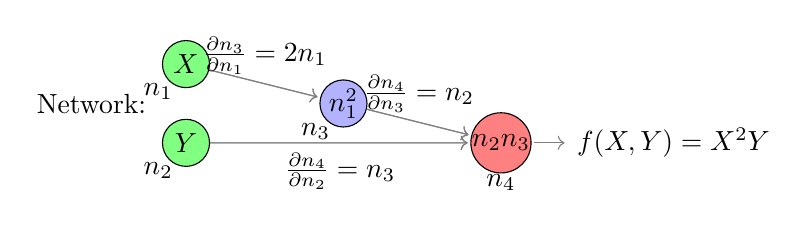
\begin{tikzpicture}[shorten >=1pt,->,draw=black!50, node distance=\layersep]
%https://tex.stackexchange.com/questions/96846/how-to-place-label-in-middle-of-line-above-and-below-with-tikz
    \tikzstyle{every pin edge}=[<-,shorten <=1pt]
    \tikzstyle{neuron}=[circle,fill=black!25,minimum size=17pt,inner sep=0pt, draw=black]
    \tikzstyle{input neuron}=[neuron, fill=green!50];
    \tikzstyle{output neuron}=[neuron, fill=red!50];
    \tikzstyle{hidden neuron}=[neuron, fill=blue!30];
    \tikzstyle{annot} = [text width=4em, text centered]


    \node[input neuron] (I-1) at (0,-1) {$X$};
    \node[input neuron] (I-2) at (0,-2) {$Y$};

    \node[hidden neuron] (H) at (2cm,-1.5 cm) {$n_1^2$};

    \node[output neuron,pin={[pin edge={->}]right:$f(X,Y) = X^2Y$}] (O) at (4cm,-2 cm) {$n_2n_3$};
    \draw (I-1) -- (H);
    \draw (H) -- (O);
    \draw (I-2) -- (O);

	\node[below left of=I-1, node distance=.5cm] {$n_1$};
	\node[below left of=I-2, node distance=.5cm] {$n_2$};
	\node[below left of=H, node distance=.5cm] {$n_3$};
	\node[below of=O, node distance=.5cm] {$n_4$};

	\node[] at (-1.2cm,-1.5cm) {Network:};

    \draw (I-1) -- node[above, pos=0.5] {$\frac{\partial n_3}{\partial n_1} = 2n_1$} ++ (H);
    \draw (H) -- node[above, pos=0.5] {$\frac{\partial n_4}{\partial n_3} = n_2$} ++(O);
    \draw (I-2) -- node[below, pos=0.5] {$\frac{\partial n_4}{\partial n_2} = n_3$} ++ (O);
\end{tikzpicture}
  \end{minipage}
  \vfill
\begin{minipage}[t][0.5\textheight][t]{\textwidth}
First, denote the value of each node by $n_i$. Second, propagating the node values through, compute the partial derivative at each connection. This can be done locally at each node upon constructing the graph.
\end{minipage}
\end{frame}



\begin{frame}[fragile]{Reverse Autodiff}
  \begin{minipage}[t][0.5\textheight][t]{\textwidth}\centering
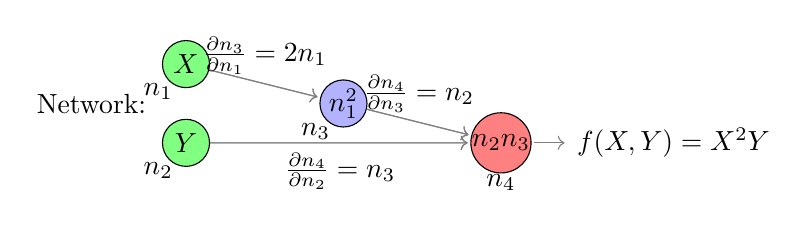
\begin{tikzpicture}[shorten >=1pt,->,draw=black!50, node distance=\layersep]
%https://tex.stackexchange.com/questions/96846/how-to-place-label-in-middle-of-line-above-and-below-with-tikz
    \tikzstyle{every pin edge}=[<-,shorten <=1pt]
    \tikzstyle{neuron}=[circle,fill=black!25,minimum size=17pt,inner sep=0pt, draw=black]
    \tikzstyle{input neuron}=[neuron, fill=green!50];
    \tikzstyle{output neuron}=[neuron, fill=red!50];
    \tikzstyle{hidden neuron}=[neuron, fill=blue!30];
    \tikzstyle{annot} = [text width=4em, text centered]


    \node[input neuron] (I-1) at (0,-1) {$X$};
    \node[input neuron] (I-2) at (0,-2) {$Y$};

    \node[hidden neuron] (H) at (2cm,-1.5 cm) {$n_1^2$};

    \node[output neuron,pin={[pin edge={->}]right:$f(X,Y) = X^2Y$}] (O) at (4cm,-2 cm) {$n_2n_3$};
    \draw (I-1) -- (H);
    \draw (H) -- (O);
    \draw (I-2) -- (O);

	\node[below left of=I-1, node distance=.5cm] {$n_1$};
	\node[below left of=I-2, node distance=.5cm] {$n_2$};
	\node[below left of=H, node distance=.5cm] {$n_3$};
	\node[below of=O, node distance=.5cm] {$n_4$};

	\node[] at (-1.2cm,-1.5cm) {Network:};

    \draw (I-1) -- node[above, pos=0.5] {$\frac{\partial n_3}{\partial n_1} = 2n_1$} ++ (H);
    \draw (H) -- node[above, pos=0.5] {$\frac{\partial n_4}{\partial n_3} = n_2$} ++(O);
    \draw (I-2) -- node[below, pos=0.5] {$\frac{\partial n_4}{\partial n_2} = n_3$} ++ (O);
\end{tikzpicture}

  \end{minipage}
  \vfill
\begin{minipage}[t][0.5\textheight][t]{\textwidth}
First, denote the value of each node by $n_i$. Second, propagating the node values through, compute the partial derivative at each connection. This can be done locally at each node upon constructing the graph. This constructs the gradient graph. 
\end{minipage}
\end{frame}




\begin{frame}[fragile]{Reverse Autodiff}
  \begin{minipage}[t][0.5\textheight][t]{\textwidth}\centering
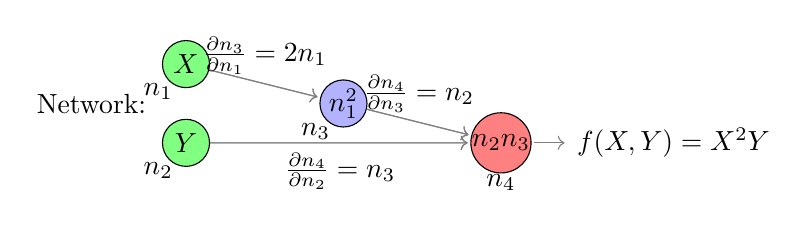
\begin{tikzpicture}[shorten >=1pt,->,draw=black!50, node distance=\layersep]
%https://tex.stackexchange.com/questions/96846/how-to-place-label-in-middle-of-line-above-and-below-with-tikz
    \tikzstyle{every pin edge}=[<-,shorten <=1pt]
    \tikzstyle{neuron}=[circle,fill=black!25,minimum size=17pt,inner sep=0pt, draw=black]
    \tikzstyle{input neuron}=[neuron, fill=green!50];
    \tikzstyle{output neuron}=[neuron, fill=red!50];
    \tikzstyle{hidden neuron}=[neuron, fill=blue!30];
    \tikzstyle{annot} = [text width=4em, text centered]


    \node[input neuron] (I-1) at (0,-1) {$X$};
    \node[input neuron] (I-2) at (0,-2) {$Y$};

    \node[hidden neuron] (H) at (2cm,-1.5 cm) {$n_1^2$};

    \node[output neuron,pin={[pin edge={->}]right:$f(X,Y) = X^2Y$}] (O) at (4cm,-2 cm) {$n_2n_3$};
    \draw (I-1) -- (H);
    \draw (H) -- (O);
    \draw (I-2) -- (O);

	\node[below left of=I-1, node distance=.5cm] {$n_1$};
	\node[below left of=I-2, node distance=.5cm] {$n_2$};
	\node[below left of=H, node distance=.5cm] {$n_3$};
	\node[below of=O, node distance=.5cm] {$n_4$};

	\node[] at (-1.2cm,-1.5cm) {Network:};

    \draw (I-1) -- node[above, pos=0.5] {$\frac{\partial n_3}{\partial n_1} = 2n_1$} ++ (H);
    \draw (H) -- node[above, pos=0.5] {$\frac{\partial n_4}{\partial n_3} = n_2$} ++(O);
    \draw (I-2) -- node[below, pos=0.5] {$\frac{\partial n_4}{\partial n_2} = n_3$} ++ (O);
\end{tikzpicture}

  \end{minipage}
  \vfill
\begin{minipage}[t][0.5\textheight][t]{\textwidth}
At runtime, for fixed $(X,Y)$, say (4,3), we compute the gradient as follows. Pass (4,3) through the graph, filling all nodes. 
\end{minipage}
\end{frame}


\begin{frame}[fragile]{Reverse Autodiff}
  \begin{minipage}[t][0.5\textheight][t]{\textwidth}\centering
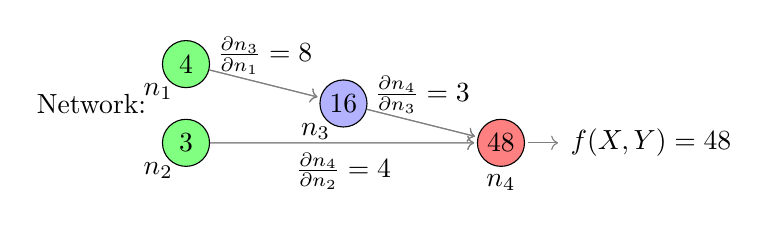
\begin{tikzpicture}[shorten >=1pt,->,draw=black!50, node distance=\layersep]
%https://tex.stackexchange.com/questions/96846/how-to-place-label-in-middle-of-line-above-and-below-with-tikz
    \tikzstyle{every pin edge}=[<-,shorten <=1pt]
    \tikzstyle{neuron}=[circle,fill=black!25,minimum size=17pt,inner sep=0pt, draw=black]
    \tikzstyle{input neuron}=[neuron, fill=green!50];
    \tikzstyle{output neuron}=[neuron, fill=red!50];
    \tikzstyle{hidden neuron}=[neuron, fill=blue!30];
    \tikzstyle{annot} = [text width=4em, text centered]


    \node[input neuron] (I-1) at (0,-1) {$4$};
    \node[input neuron] (I-2) at (0,-2) {$3$};

    \node[hidden neuron] (H) at (2cm,-1.5 cm) {$16$};

    \node[output neuron,pin={[pin edge={->}]right:$f(X,Y) = 48$}] (O) at (4cm,-2 cm) {$48$};
    \draw (I-1) -- (H);
    \draw (H) -- (O);
    \draw (I-2) -- (O);

	\node[below left of=I-1, node distance=.5cm] {$n_1$};
	\node[below left of=I-2, node distance=.5cm] {$n_2$};
	\node[below left of=H, node distance=.5cm] {$n_3$};
	\node[below of=O, node distance=.5cm] {$n_4$};

	\node[] at (-1.2cm,-1.5cm) {Network:};

    \draw (I-1) -- node[above, pos=0.5] {$\frac{\partial n_3}{\partial n_1} = 8$} ++ (H);
    \draw (H) -- node[above, pos=0.5] {$\frac{\partial n_4}{\partial n_3} = 3$} ++(O);
    \draw (I-2) -- node[below, pos=0.5] {$\frac{\partial n_4}{\partial n_2} = 4$} ++ (O);
\end{tikzpicture}

  \end{minipage}
  \vfill
\begin{minipage}[t][0.5\textheight][t]{\textwidth}
At runtime, for fixed $(X,Y)$, say (4,3), we compute the gradient as follows. Pass (4,3) through the graph, filling all nodes. 
\end{minipage}
\end{frame}



\begin{frame}[fragile]{Reverse Autodiff}
  \begin{minipage}[t][0.5\textheight][t]{\textwidth}\centering
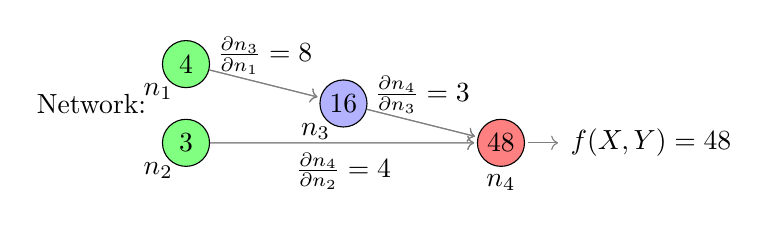
\begin{tikzpicture}[shorten >=1pt,->,draw=black!50, node distance=\layersep]
%https://tex.stackexchange.com/questions/96846/how-to-place-label-in-middle-of-line-above-and-below-with-tikz
    \tikzstyle{every pin edge}=[<-,shorten <=1pt]
    \tikzstyle{neuron}=[circle,fill=black!25,minimum size=17pt,inner sep=0pt, draw=black]
    \tikzstyle{input neuron}=[neuron, fill=green!50];
    \tikzstyle{output neuron}=[neuron, fill=red!50];
    \tikzstyle{hidden neuron}=[neuron, fill=blue!30];
    \tikzstyle{annot} = [text width=4em, text centered]


    \node[input neuron] (I-1) at (0,-1) {$4$};
    \node[input neuron] (I-2) at (0,-2) {$3$};

    \node[hidden neuron] (H) at (2cm,-1.5 cm) {$16$};

    \node[output neuron,pin={[pin edge={->}]right:$f(X,Y) = 48$}] (O) at (4cm,-2 cm) {$48$};
    \draw (I-1) -- (H);
    \draw (H) -- (O);
    \draw (I-2) -- (O);

	\node[below left of=I-1, node distance=.5cm] {$n_1$};
	\node[below left of=I-2, node distance=.5cm] {$n_2$};
	\node[below left of=H, node distance=.5cm] {$n_3$};
	\node[below of=O, node distance=.5cm] {$n_4$};

	\node[] at (-1.2cm,-1.5cm) {Network:};

    \draw (I-1) -- node[above, pos=0.5] {$\frac{\partial n_3}{\partial n_1} = 8$} ++ (H);
    \draw (H) -- node[above, pos=0.5] {$\frac{\partial n_4}{\partial n_3} = 3$} ++(O);
    \draw (I-2) -- node[below, pos=0.5] {$\frac{\partial n_4}{\partial n_2} = 4$} ++ (O);
\end{tikzpicture}

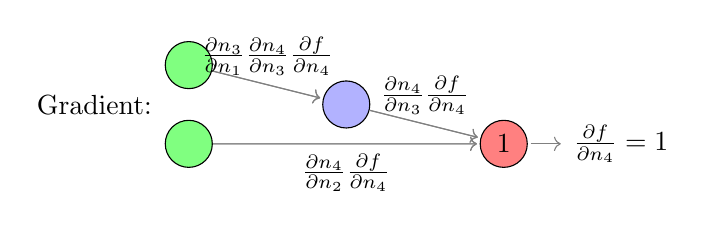
\begin{tikzpicture}[shorten >=1pt,->,draw=black!50, node distance=\layersep]
%https://tex.stackexchange.com/questions/96846/how-to-place-label-in-middle-of-line-above-and-below-with-tikz
    \tikzstyle{every pin edge}=[<-,shorten <=1pt]
    \tikzstyle{neuron}=[circle,fill=black!25,minimum size=17pt,inner sep=0pt, draw=black]
    \tikzstyle{input neuron}=[neuron, fill=green!50];
    \tikzstyle{output neuron}=[neuron, fill=red!50];
    \tikzstyle{hidden neuron}=[neuron, fill=blue!30];
    \tikzstyle{annot} = [text width=4em, text centered]


    \node[input neuron] (I-1) at (0,-1) {$$};
    \node[input neuron] (I-2) at (0,-2) {$$};

    \node[hidden neuron] (H) at (2cm,-1.5 cm) {$$};

    \node[output neuron,pin={[pin edge={->}]right:$\frac{\partial f}{\partial n_4} = 1$}] (O) at (4cm,-2 cm) {$1$};
    \draw (I-1) -- (H);
    \draw (H) -- (O);
    \draw (I-2) -- (O);

	\node[] at (-1.2cm,-1.5cm) {Gradient:};

    \draw (I-1) -- node[above, pos=0.5] {$\frac{\partial n_3}{\partial n_1}\frac{\partial n_4}{\partial n_3}\frac{\partial f}{\partial n_4} $} ++ (H);
    \draw (H) -- node[above, pos=0.5] {$\frac{\partial n_4}{\partial n_3}\frac{\partial f}{\partial n_4} $} ++(O);
    \draw (I-2) -- node[below, pos=0.5] {$\frac{\partial n_4}{\partial n_2} \frac{\partial f}{\partial n_4} $} ++ (O);
\end{tikzpicture}\hspace{2.5em}
  \end{minipage}
  \vfill
\begin{minipage}[t][0.5\textheight][t]{\textwidth}
At runtime, for fixed $(X,Y)$, say (4,3), we compute the gradient as follows. Pass (4,3) through the graph, filling all nodes. 

Second, introduce a new graph and back fill it using the values computed in the forward graph. Starting with $\frac{\partial f}{\partial n_4}  = 1$, multiply backwards until the graph is filled. 
\end{minipage}
\end{frame}



\begin{frame}[fragile]{Reverse Autodiff}
  \begin{minipage}[t][0.5\textheight][t]{\textwidth}\centering
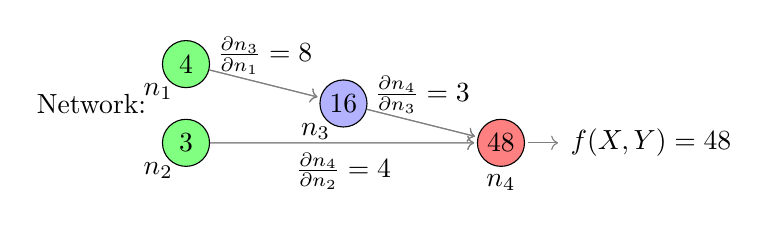
\begin{tikzpicture}[shorten >=1pt,->,draw=black!50, node distance=\layersep]
%https://tex.stackexchange.com/questions/96846/how-to-place-label-in-middle-of-line-above-and-below-with-tikz
    \tikzstyle{every pin edge}=[<-,shorten <=1pt]
    \tikzstyle{neuron}=[circle,fill=black!25,minimum size=17pt,inner sep=0pt, draw=black]
    \tikzstyle{input neuron}=[neuron, fill=green!50];
    \tikzstyle{output neuron}=[neuron, fill=red!50];
    \tikzstyle{hidden neuron}=[neuron, fill=blue!30];
    \tikzstyle{annot} = [text width=4em, text centered]


    \node[input neuron] (I-1) at (0,-1) {$4$};
    \node[input neuron] (I-2) at (0,-2) {$3$};

    \node[hidden neuron] (H) at (2cm,-1.5 cm) {$16$};

    \node[output neuron,pin={[pin edge={->}]right:$f(X,Y) = 48$}] (O) at (4cm,-2 cm) {$48$};
    \draw (I-1) -- (H);
    \draw (H) -- (O);
    \draw (I-2) -- (O);

	\node[below left of=I-1, node distance=.5cm] {$n_1$};
	\node[below left of=I-2, node distance=.5cm] {$n_2$};
	\node[below left of=H, node distance=.5cm] {$n_3$};
	\node[below of=O, node distance=.5cm] {$n_4$};

	\node[] at (-1.2cm,-1.5cm) {Network:};

    \draw (I-1) -- node[above, pos=0.5] {$\frac{\partial n_3}{\partial n_1} = 8$} ++ (H);
    \draw (H) -- node[above, pos=0.5] {$\frac{\partial n_4}{\partial n_3} = 3$} ++(O);
    \draw (I-2) -- node[below, pos=0.5] {$\frac{\partial n_4}{\partial n_2} = 4$} ++ (O);
\end{tikzpicture}

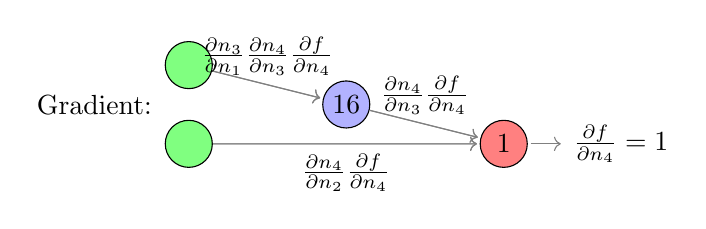
\begin{tikzpicture}[shorten >=1pt,->,draw=black!50, node distance=\layersep]
%https://tex.stackexchange.com/questions/96846/how-to-place-label-in-middle-of-line-above-and-below-with-tikz
    \tikzstyle{every pin edge}=[<-,shorten <=1pt]
    \tikzstyle{neuron}=[circle,fill=black!25,minimum size=17pt,inner sep=0pt, draw=black]
    \tikzstyle{input neuron}=[neuron, fill=green!50];
    \tikzstyle{output neuron}=[neuron, fill=red!50];
    \tikzstyle{hidden neuron}=[neuron, fill=blue!30];
    \tikzstyle{annot} = [text width=4em, text centered]


    \node[input neuron] (I-1) at (0,-1) {$$};
    \node[input neuron] (I-2) at (0,-2) {$$};

    \node[hidden neuron] (H) at (2cm,-1.5 cm) {$16$};

    \node[output neuron,pin={[pin edge={->}]right:$\frac{\partial f}{\partial n_4} = 1$}] (O) at (4cm,-2 cm) {$1$};
    \draw (I-1) -- (H);
    \draw (H) -- (O);
    \draw (I-2) -- (O);

	\node[] at (-1.2cm,-1.5cm) {Gradient:};

    \draw (I-1) -- node[above, pos=0.5] {$\frac{\partial n_3}{\partial n_1}\frac{\partial n_4}{\partial n_3}\frac{\partial f}{\partial n_4} $} ++ (H);
    \draw (H) -- node[above, pos=0.5] {$\frac{\partial n_4}{\partial n_3}\frac{\partial f}{\partial n_4} $} ++(O);
    \draw (I-2) -- node[below, pos=0.5] {$\frac{\partial n_4}{\partial n_2} \frac{\partial f}{\partial n_4} $} ++ (O);
\end{tikzpicture}\hspace{2.5em}
  \end{minipage}
  \vfill
\begin{minipage}[t][0.5\textheight][t]{\textwidth}
At runtime, for fixed $(X,Y)$, say (4,3), we compute the gradient as follows. Pass (4,3) through the graph, filling all nodes. 

Second, introduce a new graph and back fill it using the values computed in the forward graph. Starting with $\frac{\partial f}{\partial n_4}  = 1$, multiply backwards until the graph is filled. 
\end{minipage}
\end{frame}





\begin{frame}[fragile]{Reverse Autodiff}
  \begin{minipage}[t][0.5\textheight][t]{\textwidth}\centering
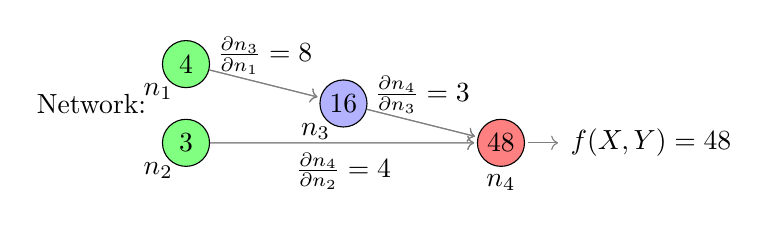
\begin{tikzpicture}[shorten >=1pt,->,draw=black!50, node distance=\layersep]
%https://tex.stackexchange.com/questions/96846/how-to-place-label-in-middle-of-line-above-and-below-with-tikz
    \tikzstyle{every pin edge}=[<-,shorten <=1pt]
    \tikzstyle{neuron}=[circle,fill=black!25,minimum size=17pt,inner sep=0pt, draw=black]
    \tikzstyle{input neuron}=[neuron, fill=green!50];
    \tikzstyle{output neuron}=[neuron, fill=red!50];
    \tikzstyle{hidden neuron}=[neuron, fill=blue!30];
    \tikzstyle{annot} = [text width=4em, text centered]


    \node[input neuron] (I-1) at (0,-1) {$4$};
    \node[input neuron] (I-2) at (0,-2) {$3$};

    \node[hidden neuron] (H) at (2cm,-1.5 cm) {$16$};

    \node[output neuron,pin={[pin edge={->}]right:$f(X,Y) = 48$}] (O) at (4cm,-2 cm) {$48$};
    \draw (I-1) -- (H);
    \draw (H) -- (O);
    \draw (I-2) -- (O);

	\node[below left of=I-1, node distance=.5cm] {$n_1$};
	\node[below left of=I-2, node distance=.5cm] {$n_2$};
	\node[below left of=H, node distance=.5cm] {$n_3$};
	\node[below of=O, node distance=.5cm] {$n_4$};

	\node[] at (-1.2cm,-1.5cm) {Network:};

    \draw (I-1) -- node[above, pos=0.5] {$\frac{\partial n_3}{\partial n_1} = 8$} ++ (H);
    \draw (H) -- node[above, pos=0.5] {$\frac{\partial n_4}{\partial n_3} = 3$} ++(O);
    \draw (I-2) -- node[below, pos=0.5] {$\frac{\partial n_4}{\partial n_2} = 4$} ++ (O);
\end{tikzpicture}

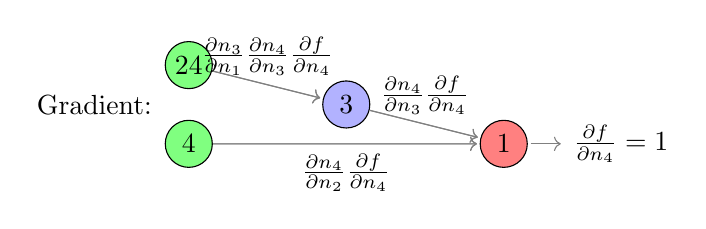
\begin{tikzpicture}[shorten >=1pt,->,draw=black!50, node distance=\layersep]
%https://tex.stackexchange.com/questions/96846/how-to-place-label-in-middle-of-line-above-and-below-with-tikz
    \tikzstyle{every pin edge}=[<-,shorten <=1pt]
    \tikzstyle{neuron}=[circle,fill=black!25,minimum size=17pt,inner sep=0pt, draw=black]
    \tikzstyle{input neuron}=[neuron, fill=green!50];
    \tikzstyle{output neuron}=[neuron, fill=red!50];
    \tikzstyle{hidden neuron}=[neuron, fill=blue!30];
    \tikzstyle{annot} = [text width=4em, text centered]


    \node[input neuron] (I-1) at (0,-1) {$24$};
    \node[input neuron] (I-2) at (0,-2) {$4$};

    \node[hidden neuron] (H) at (2cm,-1.5 cm) {$3$};

    \node[output neuron,pin={[pin edge={->}]right:$\frac{\partial f}{\partial n_4} = 1$}] (O) at (4cm,-2 cm) {$1$};
    \draw (I-1) -- (H);
    \draw (H) -- (O);
    \draw (I-2) -- (O);

	\node[] at (-1.2cm,-1.5cm) {Gradient:};

    \draw (I-1) -- node[above, pos=0.5] {$\frac{\partial n_3}{\partial n_1}\frac{\partial n_4}{\partial n_3}\frac{\partial f}{\partial n_4} $} ++ (H);
    \draw (H) -- node[above, pos=0.5] {$\frac{\partial n_4}{\partial n_3}\frac{\partial f}{\partial n_4} $} ++(O);
    \draw (I-2) -- node[below, pos=0.5] {$\frac{\partial n_4}{\partial n_2} \frac{\partial f}{\partial n_4} $} ++ (O);
\end{tikzpicture}\hspace{2.5em}
  \end{minipage}
  \vfill
\begin{minipage}[t][0.5\textheight][t]{\textwidth}
At runtime, for fixed $(X,Y)$, say (4,3), we compute the gradient as follows. Pass (4,3) through the graph, filling all nodes. 

Second, introduce a new graph and back fill it using the values computed in the forward graph. Starting with $\frac{\partial f}{\partial n_4}  = 1$, multiply backwards until the graph is filled. 
\end{minipage}
\end{frame}



\begin{frame}[fragile]{Reverse Autodiff}
  \begin{minipage}[t][0.5\textheight][t]{\textwidth}\centering
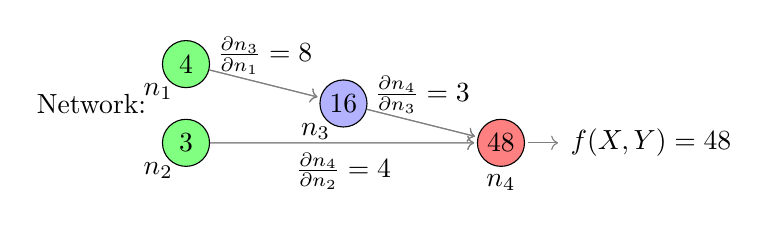
\begin{tikzpicture}[shorten >=1pt,->,draw=black!50, node distance=\layersep]
%https://tex.stackexchange.com/questions/96846/how-to-place-label-in-middle-of-line-above-and-below-with-tikz
    \tikzstyle{every pin edge}=[<-,shorten <=1pt]
    \tikzstyle{neuron}=[circle,fill=black!25,minimum size=17pt,inner sep=0pt, draw=black]
    \tikzstyle{input neuron}=[neuron, fill=green!50];
    \tikzstyle{output neuron}=[neuron, fill=red!50];
    \tikzstyle{hidden neuron}=[neuron, fill=blue!30];
    \tikzstyle{annot} = [text width=4em, text centered]


    \node[input neuron] (I-1) at (0,-1) {$4$};
    \node[input neuron] (I-2) at (0,-2) {$3$};

    \node[hidden neuron] (H) at (2cm,-1.5 cm) {$16$};

    \node[output neuron,pin={[pin edge={->}]right:$f(X,Y) = 48$}] (O) at (4cm,-2 cm) {$48$};
    \draw (I-1) -- (H);
    \draw (H) -- (O);
    \draw (I-2) -- (O);

	\node[below left of=I-1, node distance=.5cm] {$n_1$};
	\node[below left of=I-2, node distance=.5cm] {$n_2$};
	\node[below left of=H, node distance=.5cm] {$n_3$};
	\node[below of=O, node distance=.5cm] {$n_4$};

	\node[] at (-1.2cm,-1.5cm) {Network:};

    \draw (I-1) -- node[above, pos=0.5] {$\frac{\partial n_3}{\partial n_1} = 8$} ++ (H);
    \draw (H) -- node[above, pos=0.5] {$\frac{\partial n_4}{\partial n_3} = 3$} ++(O);
    \draw (I-2) -- node[below, pos=0.5] {$\frac{\partial n_4}{\partial n_2} = 4$} ++ (O);
\end{tikzpicture}

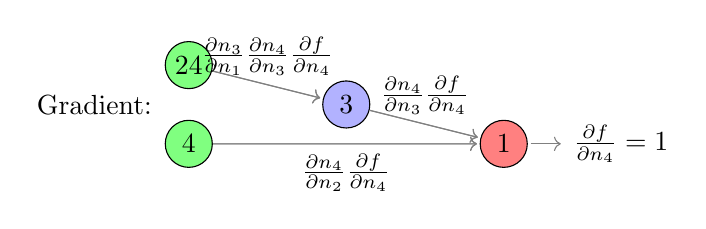
\begin{tikzpicture}[shorten >=1pt,->,draw=black!50, node distance=\layersep]
%https://tex.stackexchange.com/questions/96846/how-to-place-label-in-middle-of-line-above-and-below-with-tikz
    \tikzstyle{every pin edge}=[<-,shorten <=1pt]
    \tikzstyle{neuron}=[circle,fill=black!25,minimum size=17pt,inner sep=0pt, draw=black]
    \tikzstyle{input neuron}=[neuron, fill=green!50];
    \tikzstyle{output neuron}=[neuron, fill=red!50];
    \tikzstyle{hidden neuron}=[neuron, fill=blue!30];
    \tikzstyle{annot} = [text width=4em, text centered]


    \node[input neuron] (I-1) at (0,-1) {$24$};
    \node[input neuron] (I-2) at (0,-2) {$4$};

    \node[hidden neuron] (H) at (2cm,-1.5 cm) {$3$};

    \node[output neuron,pin={[pin edge={->}]right:$\frac{\partial f}{\partial n_4} = 1$}] (O) at (4cm,-2 cm) {$1$};
    \draw (I-1) -- (H);
    \draw (H) -- (O);
    \draw (I-2) -- (O);

	\node[] at (-1.2cm,-1.5cm) {Gradient:};

    \draw (I-1) -- node[above, pos=0.5] {$\frac{\partial n_3}{\partial n_1}\frac{\partial n_4}{\partial n_3}\frac{\partial f}{\partial n_4} $} ++ (H);
    \draw (H) -- node[above, pos=0.5] {$\frac{\partial n_4}{\partial n_3}\frac{\partial f}{\partial n_4} $} ++(O);
    \draw (I-2) -- node[below, pos=0.5] {$\frac{\partial n_4}{\partial n_2} \frac{\partial f}{\partial n_4} $} ++ (O);
\end{tikzpicture}\hspace{2.5em}
  \end{minipage}
  \vfill
\begin{minipage}[t][0.5\textheight][t]{\textwidth}
We are just computing the chain rule
$$
\frac{\partial f}{\partial X}(4,3) = \frac{\partial n_1}{\partial x} \frac{\partial n_3}{\partial n_1}\frac{\partial n_4}{\partial n_3}\frac{\partial f}{\partial n_4} (4,3) = 24
$$\pause

By precomputing the derivatives at each node, reverse autodiff allows us to very quickly compute the whole gradient in two passes though the graph. 
\end{minipage}
\end{frame}



\begin{frame}[fragile]{Reverse Autodiff}
  \begin{minipage}[t][0.5\textheight][t]{\textwidth}\centering
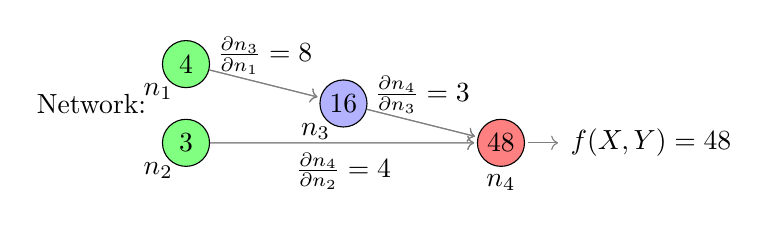
\begin{tikzpicture}[shorten >=1pt,->,draw=black!50, node distance=\layersep]
%https://tex.stackexchange.com/questions/96846/how-to-place-label-in-middle-of-line-above-and-below-with-tikz
    \tikzstyle{every pin edge}=[<-,shorten <=1pt]
    \tikzstyle{neuron}=[circle,fill=black!25,minimum size=17pt,inner sep=0pt, draw=black]
    \tikzstyle{input neuron}=[neuron, fill=green!50];
    \tikzstyle{output neuron}=[neuron, fill=red!50];
    \tikzstyle{hidden neuron}=[neuron, fill=blue!30];
    \tikzstyle{annot} = [text width=4em, text centered]


    \node[input neuron] (I-1) at (0,-1) {$4$};
    \node[input neuron] (I-2) at (0,-2) {$3$};

    \node[hidden neuron] (H) at (2cm,-1.5 cm) {$16$};

    \node[output neuron,pin={[pin edge={->}]right:$f(X,Y) = 48$}] (O) at (4cm,-2 cm) {$48$};
    \draw (I-1) -- (H);
    \draw (H) -- (O);
    \draw (I-2) -- (O);

	\node[below left of=I-1, node distance=.5cm] {$n_1$};
	\node[below left of=I-2, node distance=.5cm] {$n_2$};
	\node[below left of=H, node distance=.5cm] {$n_3$};
	\node[below of=O, node distance=.5cm] {$n_4$};

	\node[] at (-1.2cm,-1.5cm) {Network:};

    \draw (I-1) -- node[above, pos=0.5] {$\frac{\partial n_3}{\partial n_1} = 8$} ++ (H);
    \draw (H) -- node[above, pos=0.5] {$\frac{\partial n_4}{\partial n_3} = 3$} ++(O);
    \draw (I-2) -- node[below, pos=0.5] {$\frac{\partial n_4}{\partial n_2} = 4$} ++ (O);
\end{tikzpicture}

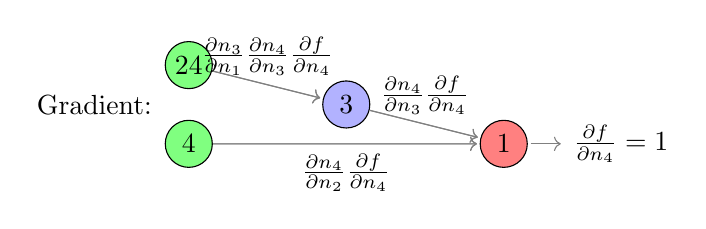
\begin{tikzpicture}[shorten >=1pt,->,draw=black!50, node distance=\layersep]
%https://tex.stackexchange.com/questions/96846/how-to-place-label-in-middle-of-line-above-and-below-with-tikz
    \tikzstyle{every pin edge}=[<-,shorten <=1pt]
    \tikzstyle{neuron}=[circle,fill=black!25,minimum size=17pt,inner sep=0pt, draw=black]
    \tikzstyle{input neuron}=[neuron, fill=green!50];
    \tikzstyle{output neuron}=[neuron, fill=red!50];
    \tikzstyle{hidden neuron}=[neuron, fill=blue!30];
    \tikzstyle{annot} = [text width=4em, text centered]


    \node[input neuron] (I-1) at (0,-1) {$24$};
    \node[input neuron] (I-2) at (0,-2) {$4$};

    \node[hidden neuron] (H) at (2cm,-1.5 cm) {$3$};

    \node[output neuron,pin={[pin edge={->}]right:$\frac{\partial f}{\partial n_4} = 1$}] (O) at (4cm,-2 cm) {$1$};
    \draw (I-1) -- (H);
    \draw (H) -- (O);
    \draw (I-2) -- (O);

	\node[] at (-1.2cm,-1.5cm) {Gradient:};

    \draw (I-1) -- node[above, pos=0.5] {$\frac{\partial n_3}{\partial n_1}\frac{\partial n_4}{\partial n_3}\frac{\partial f}{\partial n_4} $} ++ (H);
    \draw (H) -- node[above, pos=0.5] {$\frac{\partial n_4}{\partial n_3}\frac{\partial f}{\partial n_4} $} ++(O);
    \draw (I-2) -- node[below, pos=0.5] {$\frac{\partial n_4}{\partial n_2} \frac{\partial f}{\partial n_4} $} ++ (O);
\end{tikzpicture}\hspace{2.5em}
  \end{minipage}
  \vfill
\begin{minipage}[t][0.5\textheight][t]{\textwidth}
There is of course one caveat: If we have many output labels $f_i$ or a node that is not differentiable we may not be able to use reverse autodiff. \pause

The first problem is simply an limitation of the algorithm, but the second we can often smooth away by replacing a node with a smooth function, or by using a subgradient.
\end{minipage}
\end{frame}




\begin{frame}[fragile]{Training Neural Networks}
  \begin{minipage}[t][0.5\textheight][t]{\textwidth}
	\centering \includegraphics[width=\textwidth]{L11GradientDecent.png} 
  \end{minipage}
  \vfill
\begin{minipage}[t][0.5\textheight][t]{\textwidth}
The four nontrivial methods of computing gradients for gradient decent are summarized in this tabel taken from Chapter 9 or Geron. Tensorflow has automatically implemented reverse autodiff and as long as you use it's constructors it can compute gradients for you. \pause 

If you intend to implement a new kind of neuron you will have to code in compatibility with autodiff by hand, but after you do it once tensorflow will take it forward. 
\end{minipage}

\end{frame}







\begin{frame}[fragile]{Reference}
 
McCulloch and Pitts "A logical calculus of ideas immanent is nervous activity." \url{http://www.cse.chalmers.se/~coquand/AUTOMATA/mcp.pdf}

Neuroplacsicity Picture: \url{https://www.cognifit.com/brain-plasticity-and-cognition}

This lecture is based on Chapters 9 - 10 of Geron "Hands on Machine Learning with Scikit-Learn and Tensorflow."

\end{frame}


\end{document}






\begin{frame}[fragile]{Test}
\begin{minipage}[t][0.5\textheight][t]{\textwidth}\centering
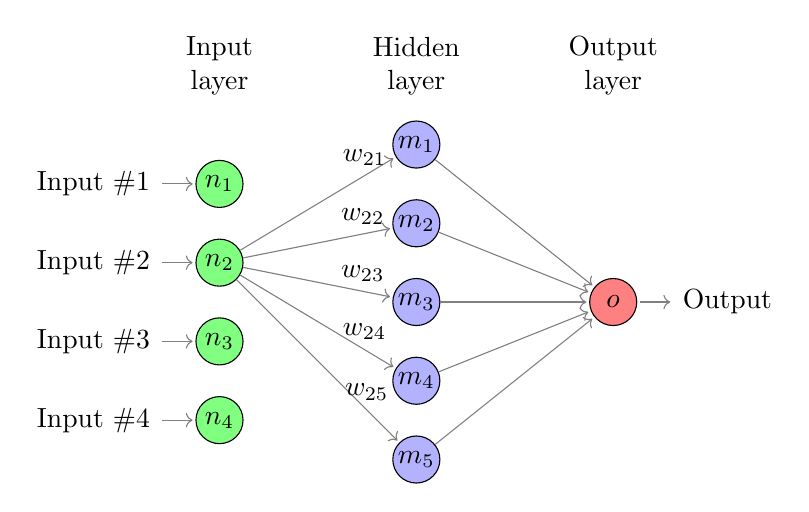
\begin{tikzpicture}[shorten >=1pt,->,draw=black!50, node distance=\layersep]
%https://tex.stackexchange.com/questions/96846/how-to-place-label-in-middle-of-line-above-and-below-with-tikz
    \tikzstyle{every pin edge}=[<-,shorten <=1pt]
    \tikzstyle{neuron}=[circle,fill=black!25,minimum size=17pt,inner sep=0pt, draw=black]
    \tikzstyle{input neuron}=[neuron, fill=green!50];
    \tikzstyle{output neuron}=[neuron, fill=red!50];
    \tikzstyle{hidden neuron}=[neuron, fill=blue!30];
    \tikzstyle{annot} = [text width=4em, text centered]

    % Draw the input layer nodes
    \foreach \name / \y in {1,...,4}
    % This is the same as writing \foreach \name / \y in {1/1,2/2,3/3,4/4}
        \node[input neuron, pin=left:Input \#\y] (I-\name) at (0,-\y) {$n_\y$};

    % Draw the hidden layer nodes
    \foreach \name / \y in {1,...,5}
        \path[yshift=0.5cm]
            node[hidden neuron] (H-\name) at (\layersep,-\y cm) {$m_\y$};

    % Draw the output layer node
    \node[output neuron,pin={[pin edge={->}]right:Output}, right of=H-3] (O) {$o$};

    % Connect every node in the input layer with every node in the
    % hidden layer.
%    \foreach \source in {1,...,4}
%        \foreach \dest in {1,...,5}
%            \draw (I-\source) -- node[below] {$w_ij$} ++ (H-\dest);


%    \foreach \source in {1,...,4}
        \foreach \dest in {1,...,5}
            \draw (I-2) -- node[above, pos=0.8] {$w_{2\dest}$} ++ (H-\dest);

    % Connect every node in the hidden layer with the output layer
    \foreach \source in {1,...,5}
        \path (H-\source) edge (O);

    % Annotate the layers
    \node[annot,above of=H-1, node distance=1cm] (hl) {Hidden layer};
    \node[annot,left of=hl] {Input layer};
    \node[annot,right of=hl] {Output layer};
\end{tikzpicture}
  \end{minipage}
  \vfill
\begin{minipage}[t][0.5\textheight][t]{\textwidth}

\end{minipage}


\end{frame}
%%%%%%%%%%%%%%%%%%%%%%%%%%%%%%%%%%%%%%%%%%%
%%%%%%%%%%%%%%%%%%%%%%%%%%%%%%%%%%%%%%%%%%%
%%%%%%%%%%%%%%%%%%%%%%%%%%%%%%%%%%%%%%%%%%%



\begin{frame}[fragile]{Introduction}

\end{frame}




\begin{frame}[fragile]{Binary Classification}
  \begin{minipage}[t][0.5\textheight][t]{\textwidth}
	\centering \includegraphics[height=0.5\textheight]{.png} 
  \end{minipage}
  \vfill
\begin{minipage}[t][0.5\textheight][t]{\textwidth}

\end{minipage}
\end{frame}



\begin{frame}[fragile]{Point Variance of Linear Predictor}

\begin{align*}
\action<+->{ &=&&}
\\
\action<+->{  &=   && }
\end{align*}
\action<+->{The}
\end{frame}



\begin{frame}[fragile]{Correlation}
\begin{itemize}
\item[] \textbf{Serial No.} is basically uncorrelated with anything. \pause
\item[] \textbf{Admit} is highly correlated with \textbf{CGPA}, \textbf{TOEFL Score} and \textbf{GRE Score}\pause
\item[] \textbf{Research} has a lowish correlation with \textbf{Admit}, but also with everything else.  
\end{itemize}
\end{frame}











\begin{frame}[fragile]{Bias, Variance and Parameters}
  \begin{minipage}[t][0.5\textheight][t]{\textwidth}
	\centering
	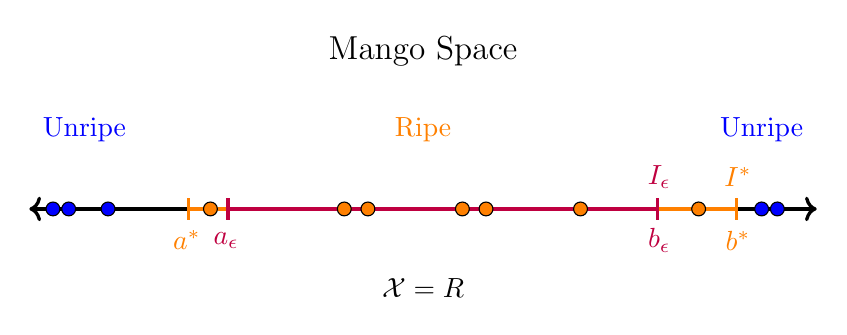
\begin{tikzpicture}
		\draw[<->,very thick] (-5,0) -- (5,0);
		\draw[color = orange, |-|,very thick] (-3,0) -- (4,0);
		\node[color=orange] at (4,.4) {$I^*$};
		\node at (0,2) {\large Mango Space} ;
		\node at (0,-1) {$\mathcal{X} = \mathbb{R}$} ;
		\node [color=blue] at (-4.3,1) {Unripe} ;
		\node [color=blue] at (4.3,1) {Unripe} ;
		\node [color=orange] at (0,1) {Ripe} ;

		\node [color=orange] at (-3,-.4) {$a^*$} ;
		\node [color=orange] at (4,-.4) {$b^*$} ;

		\draw [color=purple, |-|,very thick] (-2.5,0) -- (3,0);
		\node [color=purple] at (3,.4) {$I_\epsilon$} ;
		\node [color=purple] at (-2.5,-.4) {$a_\epsilon$} ;
		\node [color=purple] at (3,-.4) {$b_\epsilon$} ;

%		\draw [color=olive, |-|,very thick] (-3.5,0) -- (2.5,0);
%		\node [color=olive] at (3,.4) {$h_{\mathcal{T}}$} ;



		\node[circle,draw=black, fill=orange, inner sep=0pt,minimum size=5pt] at (2,0) {};
		\node[circle,draw=black, fill=orange, inner sep=0pt,minimum size=5pt] at (-1,0) {};
		\node[circle,draw=black, fill=orange, inner sep=0pt,minimum size=5pt] at (-.7,0) {};
		\node[circle,draw=black, fill=orange, inner sep=0pt,minimum size=5pt] at (.5,0) {};
		\node[circle,draw=black, fill=orange, inner sep=0pt,minimum size=5pt] at (.8,0) {};
		\node[circle,draw=black, fill=orange, inner sep=0pt,minimum size=5pt] at (-2.7,0) {};
		\node[circle,draw=black, fill=orange, inner sep=0pt,minimum size=5pt] at (3.5,0) {};

		\node[circle,draw=black, fill=blue, inner sep=0pt,minimum size=5pt] at (-4.5,0) {};
		\node[circle,draw=black, fill=blue, inner sep=0pt,minimum size=5pt] at (-4,0) {};
		\node[circle,draw=black, fill=blue, inner sep=0pt,minimum size=5pt] at (-4.7,0) {};
		\node[circle,draw=black, fill=blue, inner sep=0pt,minimum size=5pt] at (4.3,0) {};
		\node[circle,draw=black, fill=blue, inner sep=0pt,minimum size=5pt] at (4.5,0) {};
	\end{tikzpicture}
  \end{minipage}
  \vfill
  \begin{minipage}[t][0.5\textheight][t]{\textwidth}
Lets understand this visually.
$$
Err(x_0) = \sigma_\epsilon^2 + [E_\cT[\hat f(x_0)] - f(x_0)]^2 + E_\cT\big[ \hat{f}(x_0) - E_\cT[\hat{f}(x_0)] \big]^2\,.
$$\pause
Consider a data set, 
\end{minipage}
\end{frame}





























